% Options for packages loaded elsewhere
\PassOptionsToPackage{unicode}{hyperref}
\PassOptionsToPackage{hyphens}{url}
%
\documentclass[
]{article}
\usepackage{amsmath,amssymb}
\usepackage{iftex}
\ifPDFTeX
  \usepackage[T1]{fontenc}
  \usepackage[utf8]{inputenc}
  \usepackage{textcomp} % provide euro and other symbols
\else % if luatex or xetex
  \usepackage{unicode-math} % this also loads fontspec
  \defaultfontfeatures{Scale=MatchLowercase}
  \defaultfontfeatures[\rmfamily]{Ligatures=TeX,Scale=1}
\fi
\usepackage{lmodern}
\ifPDFTeX\else
  % xetex/luatex font selection
\fi
% Use upquote if available, for straight quotes in verbatim environments
\IfFileExists{upquote.sty}{\usepackage{upquote}}{}
\IfFileExists{microtype.sty}{% use microtype if available
  \usepackage[]{microtype}
  \UseMicrotypeSet[protrusion]{basicmath} % disable protrusion for tt fonts
}{}
\makeatletter
\@ifundefined{KOMAClassName}{% if non-KOMA class
  \IfFileExists{parskip.sty}{%
    \usepackage{parskip}
  }{% else
    \setlength{\parindent}{0pt}
    \setlength{\parskip}{6pt plus 2pt minus 1pt}}
}{% if KOMA class
  \KOMAoptions{parskip=half}}
\makeatother
\usepackage{xcolor}
\usepackage[margin=1in]{geometry}
\usepackage{color}
\usepackage{fancyvrb}
\newcommand{\VerbBar}{|}
\newcommand{\VERB}{\Verb[commandchars=\\\{\}]}
\DefineVerbatimEnvironment{Highlighting}{Verbatim}{commandchars=\\\{\}}
% Add ',fontsize=\small' for more characters per line
\usepackage{framed}
\definecolor{shadecolor}{RGB}{248,248,248}
\newenvironment{Shaded}{\begin{snugshade}}{\end{snugshade}}
\newcommand{\AlertTok}[1]{\textcolor[rgb]{0.94,0.16,0.16}{#1}}
\newcommand{\AnnotationTok}[1]{\textcolor[rgb]{0.56,0.35,0.01}{\textbf{\textit{#1}}}}
\newcommand{\AttributeTok}[1]{\textcolor[rgb]{0.13,0.29,0.53}{#1}}
\newcommand{\BaseNTok}[1]{\textcolor[rgb]{0.00,0.00,0.81}{#1}}
\newcommand{\BuiltInTok}[1]{#1}
\newcommand{\CharTok}[1]{\textcolor[rgb]{0.31,0.60,0.02}{#1}}
\newcommand{\CommentTok}[1]{\textcolor[rgb]{0.56,0.35,0.01}{\textit{#1}}}
\newcommand{\CommentVarTok}[1]{\textcolor[rgb]{0.56,0.35,0.01}{\textbf{\textit{#1}}}}
\newcommand{\ConstantTok}[1]{\textcolor[rgb]{0.56,0.35,0.01}{#1}}
\newcommand{\ControlFlowTok}[1]{\textcolor[rgb]{0.13,0.29,0.53}{\textbf{#1}}}
\newcommand{\DataTypeTok}[1]{\textcolor[rgb]{0.13,0.29,0.53}{#1}}
\newcommand{\DecValTok}[1]{\textcolor[rgb]{0.00,0.00,0.81}{#1}}
\newcommand{\DocumentationTok}[1]{\textcolor[rgb]{0.56,0.35,0.01}{\textbf{\textit{#1}}}}
\newcommand{\ErrorTok}[1]{\textcolor[rgb]{0.64,0.00,0.00}{\textbf{#1}}}
\newcommand{\ExtensionTok}[1]{#1}
\newcommand{\FloatTok}[1]{\textcolor[rgb]{0.00,0.00,0.81}{#1}}
\newcommand{\FunctionTok}[1]{\textcolor[rgb]{0.13,0.29,0.53}{\textbf{#1}}}
\newcommand{\ImportTok}[1]{#1}
\newcommand{\InformationTok}[1]{\textcolor[rgb]{0.56,0.35,0.01}{\textbf{\textit{#1}}}}
\newcommand{\KeywordTok}[1]{\textcolor[rgb]{0.13,0.29,0.53}{\textbf{#1}}}
\newcommand{\NormalTok}[1]{#1}
\newcommand{\OperatorTok}[1]{\textcolor[rgb]{0.81,0.36,0.00}{\textbf{#1}}}
\newcommand{\OtherTok}[1]{\textcolor[rgb]{0.56,0.35,0.01}{#1}}
\newcommand{\PreprocessorTok}[1]{\textcolor[rgb]{0.56,0.35,0.01}{\textit{#1}}}
\newcommand{\RegionMarkerTok}[1]{#1}
\newcommand{\SpecialCharTok}[1]{\textcolor[rgb]{0.81,0.36,0.00}{\textbf{#1}}}
\newcommand{\SpecialStringTok}[1]{\textcolor[rgb]{0.31,0.60,0.02}{#1}}
\newcommand{\StringTok}[1]{\textcolor[rgb]{0.31,0.60,0.02}{#1}}
\newcommand{\VariableTok}[1]{\textcolor[rgb]{0.00,0.00,0.00}{#1}}
\newcommand{\VerbatimStringTok}[1]{\textcolor[rgb]{0.31,0.60,0.02}{#1}}
\newcommand{\WarningTok}[1]{\textcolor[rgb]{0.56,0.35,0.01}{\textbf{\textit{#1}}}}
\usepackage{graphicx}
\makeatletter
\def\maxwidth{\ifdim\Gin@nat@width>\linewidth\linewidth\else\Gin@nat@width\fi}
\def\maxheight{\ifdim\Gin@nat@height>\textheight\textheight\else\Gin@nat@height\fi}
\makeatother
% Scale images if necessary, so that they will not overflow the page
% margins by default, and it is still possible to overwrite the defaults
% using explicit options in \includegraphics[width, height, ...]{}
\setkeys{Gin}{width=\maxwidth,height=\maxheight,keepaspectratio}
% Set default figure placement to htbp
\makeatletter
\def\fps@figure{htbp}
\makeatother
\setlength{\emergencystretch}{3em} % prevent overfull lines
\providecommand{\tightlist}{%
  \setlength{\itemsep}{0pt}\setlength{\parskip}{0pt}}
\setcounter{secnumdepth}{-\maxdimen} % remove section numbering
\usepackage{booktabs}
\usepackage{caption}
\usepackage{longtable}
\usepackage{colortbl}
\usepackage{array}
\usepackage{anyfontsize}
\usepackage{multirow}
\ifLuaTeX
  \usepackage{selnolig}  % disable illegal ligatures
\fi
\usepackage{bookmark}
\IfFileExists{xurl.sty}{\usepackage{xurl}}{} % add URL line breaks if available
\urlstyle{same}
\hypersetup{
  pdftitle={SDG INDICATORS CALCULATIONS - Zambia Example},
  hidelinks,
  pdfcreator={LaTeX via pandoc}}

\title{SDG INDICATORS CALCULATIONS - Zambia Example}
\author{true}
\date{}

\begin{document}
\maketitle

\subsection{INTRODUCTION}\label{introduction}

This R markdown template will take through computation of some SDG 3, 5
and 8 key indicators namely;

\begin{itemize}
\item
  SDG Indicator 3.7.2: Adolescent birth rate (aged 10--14 years; aged
  15--19 years) per 1,000 women in that age group.
\item
  SDG INDICATOR 5.3.1: Proportion of women aged 20--24 years who were
  married or in a union before age 15 and before age 18.
\item
  SDG INDICATOR 8.6.1: Proportion of youth (aged 15-24 years) not in
  education, employment or training.
\end{itemize}

\subsection{LOAD LIBRARIES}\label{load-libraries}

\begin{Shaded}
\begin{Highlighting}[]
\ControlFlowTok{if}\NormalTok{(}\SpecialCharTok{!}\FunctionTok{require}\NormalTok{(}\StringTok{"pacman"}\NormalTok{)) }\FunctionTok{install.packages}\NormalTok{(}\StringTok{"pacman"}\NormalTok{)}

\NormalTok{pacman}\SpecialCharTok{::}\FunctionTok{p\_load}\NormalTok{(tidyverse, haven, forcats, gt, sf, ggrepel, patchwork)}
\end{Highlighting}
\end{Shaded}

\subsection{LOAD DATA}\label{load-data}

This represent 10\% from the Zambia 2010 population and houses census
data whose sole purpose is for this exercise.

\begin{Shaded}
\begin{Highlighting}[]
\NormalTok{demographics }\OtherTok{\textless{}{-}}\NormalTok{ haven}\SpecialCharTok{::}\FunctionTok{read\_sav}\NormalTok{(}\StringTok{"input/DataExercise/SPSS files/DemographicsDIST.sav"}\NormalTok{)}

\NormalTok{constituency\_shape }\OtherTok{\textless{}{-}}\NormalTok{ sf}\SpecialCharTok{::}\FunctionTok{read\_sf}\NormalTok{(}\StringTok{"input/TUC/zambia\_constituency\_reproj\_pop\_GHS{-}DU{-}TUC.shp"}\NormalTok{)}
\end{Highlighting}
\end{Shaded}

\subsection{DATA DESCRIPTION \&
EXPLORATION}\label{data-description-exploration}

\textbf{Description}

There are two main datasets used in this exercise.

\begin{itemize}
\item
  \textbf{demographics} : 10\% of Zambia 2010 individual census data
  with 1,321,973 records and 92 variables. This will be used to compute
  the SDG indicators using variables such as age, sex, activity in the
  past 12 months, child bird in the past 12 months and constituency.
\item
  \textbf{constituency\_shape} : Zambia constituency boundaries (admin
  4) with 150 records and 34 variables including information on the
  DEGURBA classification. This will be used to map the SDG indicators
  computed from the demographic data and then later to disaggregate the
  indicators my DEGURBA.
\end{itemize}

\textbf{Exploration}

In this section, we are exploring the key variables that will be used in
this exercise. These variables are

\begin{itemize}
\tightlist
\item
  \emph{P4\_SEX\_P = Sex}
\end{itemize}

\begin{Shaded}
\begin{Highlighting}[]
\CommentTok{\# Sex unique values}
\NormalTok{demographics}\SpecialCharTok{$}\NormalTok{P4\_SEX\_P }\SpecialCharTok{|\textgreater{}} \FunctionTok{str}\NormalTok{()}
\end{Highlighting}
\end{Shaded}

\begin{verbatim}
##  dbl+lbl [1:1321973] 2, 2, 2, 2, 1, 2, 2, 1, 2, 2, 2, 2, 1, 1, 2, 1, 1, 1, ...
##  @ label        : chr "Sex"
##  @ format.spss  : chr "F1.0"
##  @ display_width: int 10
##  @ labels       : Named num [1:2] 1 2
##   ..- attr(*, "names")= chr [1:2] "Male" "Female"
\end{verbatim}

\begin{Shaded}
\begin{Highlighting}[]
\CommentTok{\# Sex distribution}
\NormalTok{demographics }\SpecialCharTok{|\textgreater{}}
  \FunctionTok{mutate}\NormalTok{(}\AttributeTok{P4\_SEX\_P =} \FunctionTok{as\_factor}\NormalTok{(P4\_SEX\_P)) }\SpecialCharTok{|\textgreater{}}
\NormalTok{  dplyr}\SpecialCharTok{::}\FunctionTok{group\_by}\NormalTok{(P4\_SEX\_P) }\SpecialCharTok{|\textgreater{}}
  \FunctionTok{count}\NormalTok{(}\AttributeTok{name =} \StringTok{"Freq"}\NormalTok{) }\SpecialCharTok{|\textgreater{}}
\NormalTok{  tibble}\SpecialCharTok{::}\FunctionTok{tibble}\NormalTok{() }\SpecialCharTok{|\textgreater{}}
\NormalTok{  ggplot2}\SpecialCharTok{::}\FunctionTok{ggplot}\NormalTok{() }\SpecialCharTok{+}
\NormalTok{  ggplot2}\SpecialCharTok{::}\FunctionTok{geom\_bar}\NormalTok{(}\FunctionTok{aes}\NormalTok{(}\AttributeTok{x =}\NormalTok{ P4\_SEX\_P, }\AttributeTok{fill =}\NormalTok{ P4\_SEX\_P, }\AttributeTok{y =}\NormalTok{ Freq), }
                    \AttributeTok{stat =} \StringTok{"identity"}\NormalTok{) }\SpecialCharTok{+}
\NormalTok{  ggplot2}\SpecialCharTok{::}\FunctionTok{labs}\NormalTok{(}\AttributeTok{title =} \StringTok{"Sex Distribution"}\NormalTok{) }\SpecialCharTok{+}
\NormalTok{  ggplot2}\SpecialCharTok{::}\FunctionTok{theme\_minimal}\NormalTok{()}
\end{Highlighting}
\end{Shaded}

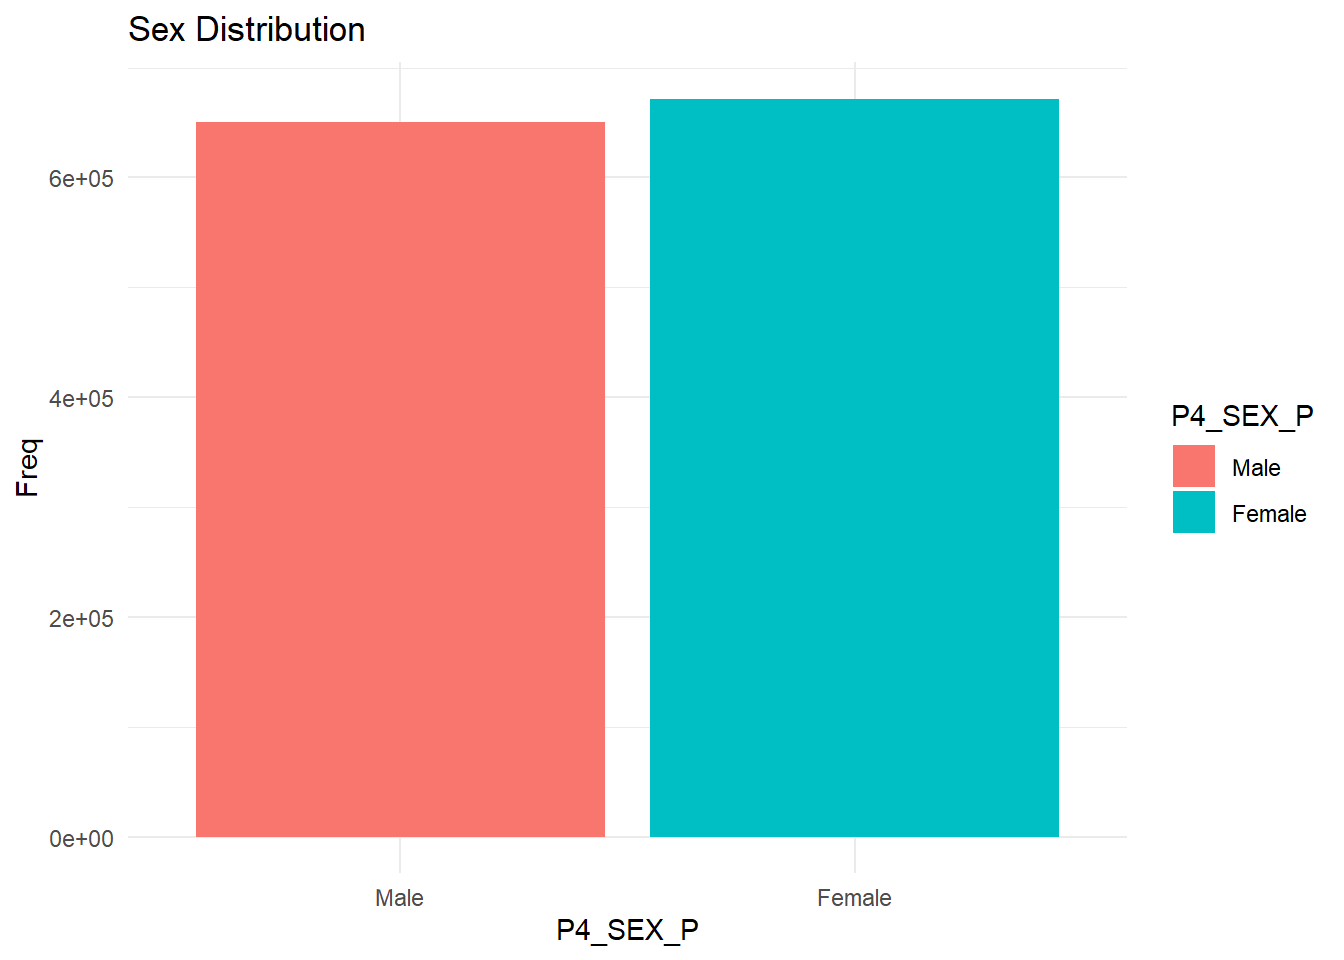
\includegraphics{indicators_notebook_files/figure-latex/unnamed-chunk-3-1.pdf}

\begin{itemize}
\tightlist
\item
  \emph{P5\_AGE\_P = Age}
\end{itemize}

\begin{Shaded}
\begin{Highlighting}[]
\CommentTok{\# Age distribution}
\NormalTok{demographics}\SpecialCharTok{$}\NormalTok{P5\_AGE\_P }\SpecialCharTok{|\textgreater{}} \FunctionTok{hist}\NormalTok{(}\AttributeTok{col =} \StringTok{"grey"}\NormalTok{, }
                              \AttributeTok{main =} \StringTok{"Age Distribution"}\NormalTok{,}
                              \AttributeTok{xlab =} \StringTok{"Age"}\NormalTok{, }
                              \AttributeTok{ylab =} \StringTok{"Count"}\NormalTok{, }
                              \AttributeTok{border =} \StringTok{"black"}\NormalTok{, }
                              \AttributeTok{breaks =} \FunctionTok{length}\NormalTok{(}\FunctionTok{unique}\NormalTok{(demographics}\SpecialCharTok{$}\NormalTok{P5\_AGE\_P)))}
\end{Highlighting}
\end{Shaded}

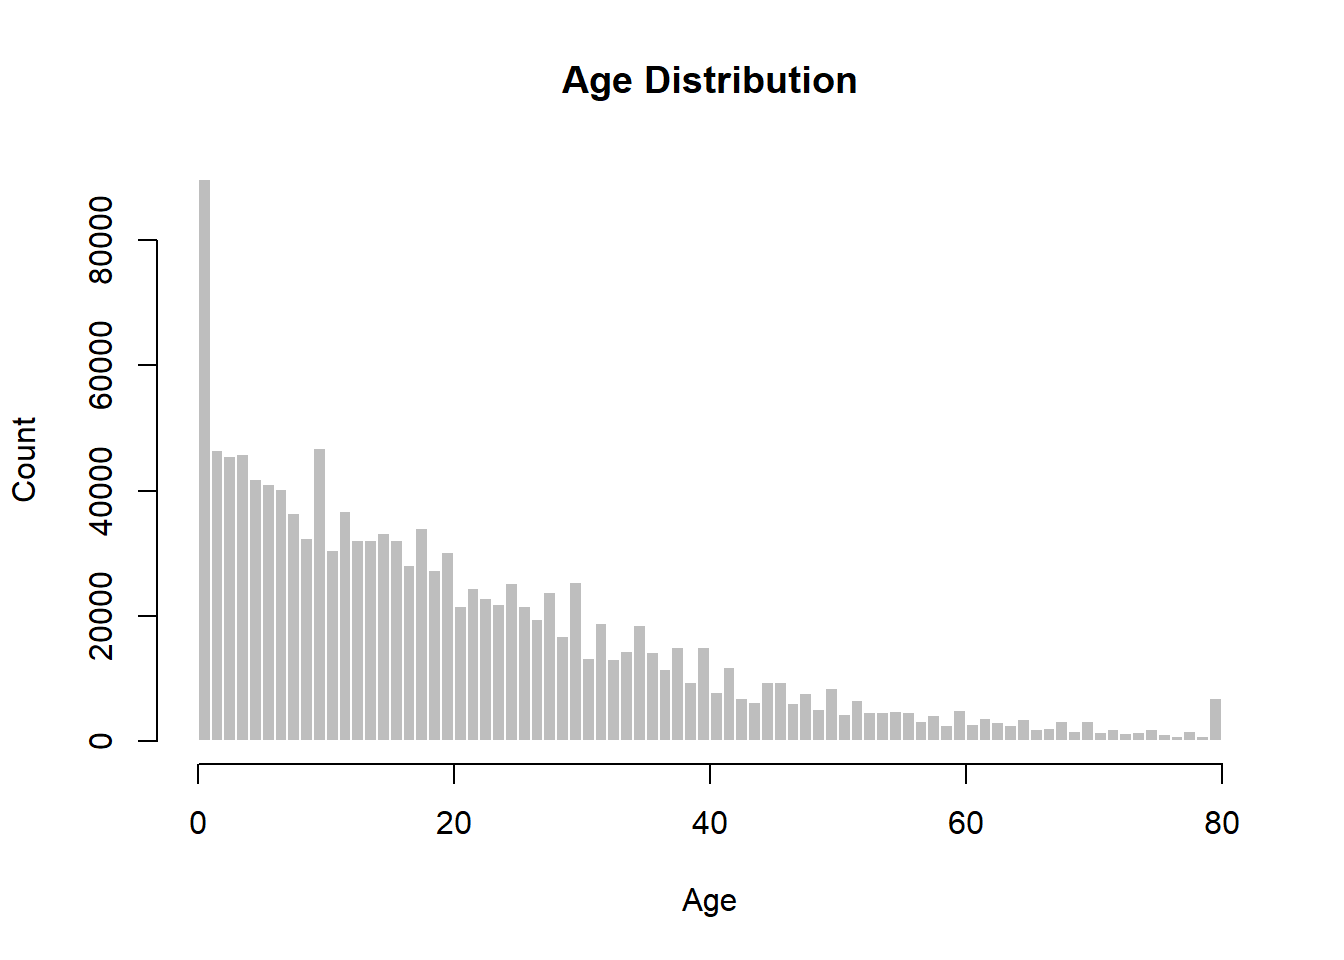
\includegraphics{indicators_notebook_files/figure-latex/unnamed-chunk-4-1.pdf}

\begin{Shaded}
\begin{Highlighting}[]
\CommentTok{\# Age distribution by Sex}
\NormalTok{demographics }\SpecialCharTok{|\textgreater{}}
  \FunctionTok{group\_by}\NormalTok{(P4\_SEX\_P, P5\_AGE\_P) }\SpecialCharTok{|\textgreater{}}
  \FunctionTok{summarise}\NormalTok{(}\AttributeTok{pop\_count =} \FunctionTok{n}\NormalTok{()}\SpecialCharTok{/}\DecValTok{10000}\NormalTok{) }\SpecialCharTok{|\textgreater{}}
  \FunctionTok{mutate}\NormalTok{(}
    \AttributeTok{pop\_count =} \FunctionTok{case\_when}\NormalTok{(}
\NormalTok{      P4\_SEX\_P }\SpecialCharTok{==} \DecValTok{1} \SpecialCharTok{\textasciitilde{}} \SpecialCharTok{{-}}\NormalTok{pop\_count,}
\NormalTok{      P4\_SEX\_P }\SpecialCharTok{==} \DecValTok{2} \SpecialCharTok{\textasciitilde{}}\NormalTok{ pop\_count}
\NormalTok{    ),}
    \AttributeTok{sex\_label =} \FunctionTok{factor}\NormalTok{(P4\_SEX\_P, }\AttributeTok{levels =} \FunctionTok{c}\NormalTok{(}\DecValTok{1}\NormalTok{, }\DecValTok{2}\NormalTok{), }\AttributeTok{labels =} \FunctionTok{c}\NormalTok{(}\StringTok{"Male"}\NormalTok{, }\StringTok{"Female"}\NormalTok{)),}
    \AttributeTok{age\_factor =} \FunctionTok{factor}\NormalTok{(P5\_AGE\_P, }\AttributeTok{levels =} \FunctionTok{sort}\NormalTok{(}\FunctionTok{unique}\NormalTok{(P5\_AGE\_P)))}
\NormalTok{  ) }\SpecialCharTok{|\textgreater{}}
\NormalTok{  ggplot2}\SpecialCharTok{::}\FunctionTok{ggplot}\NormalTok{(}\FunctionTok{aes}\NormalTok{(}\AttributeTok{x =}\NormalTok{ pop\_count, }\AttributeTok{y =}\NormalTok{ age\_factor, }\AttributeTok{fill =}\NormalTok{ sex\_label)) }\SpecialCharTok{+}
\NormalTok{  ggplot2}\SpecialCharTok{::}\FunctionTok{geom\_bar}\NormalTok{(}\AttributeTok{stat =} \StringTok{"identity"}\NormalTok{, }\AttributeTok{width =} \DecValTok{1}\NormalTok{, , }\AttributeTok{color =} \StringTok{"white"}\NormalTok{) }\SpecialCharTok{+}
\NormalTok{  ggplot2}\SpecialCharTok{::}\FunctionTok{scale\_x\_continuous}\NormalTok{(}\AttributeTok{labels =}\NormalTok{ abs) }\SpecialCharTok{+}
\NormalTok{  ggplot2}\SpecialCharTok{::}\FunctionTok{labs}\NormalTok{(}\AttributeTok{title =} \StringTok{"Age {-} Sex Distribution"}\NormalTok{,}
                \AttributeTok{x =} \StringTok{"Population Count (million)"}\NormalTok{, }
                \AttributeTok{y =} \StringTok{"Age"}\NormalTok{, }
                \AttributeTok{fill =} \StringTok{"Sex"}\NormalTok{) }\SpecialCharTok{+}
\NormalTok{  ggplot2}\SpecialCharTok{::}\FunctionTok{theme\_minimal}\NormalTok{() }\SpecialCharTok{+}
\NormalTok{  ggplot2}\SpecialCharTok{::}\FunctionTok{theme}\NormalTok{(}
    \AttributeTok{panel.grid =} \FunctionTok{element\_blank}\NormalTok{(),}
    \AttributeTok{plot.title =} \FunctionTok{element\_text}\NormalTok{(}\AttributeTok{hjust =} \FloatTok{0.5}\NormalTok{)}
\NormalTok{  )}
\end{Highlighting}
\end{Shaded}

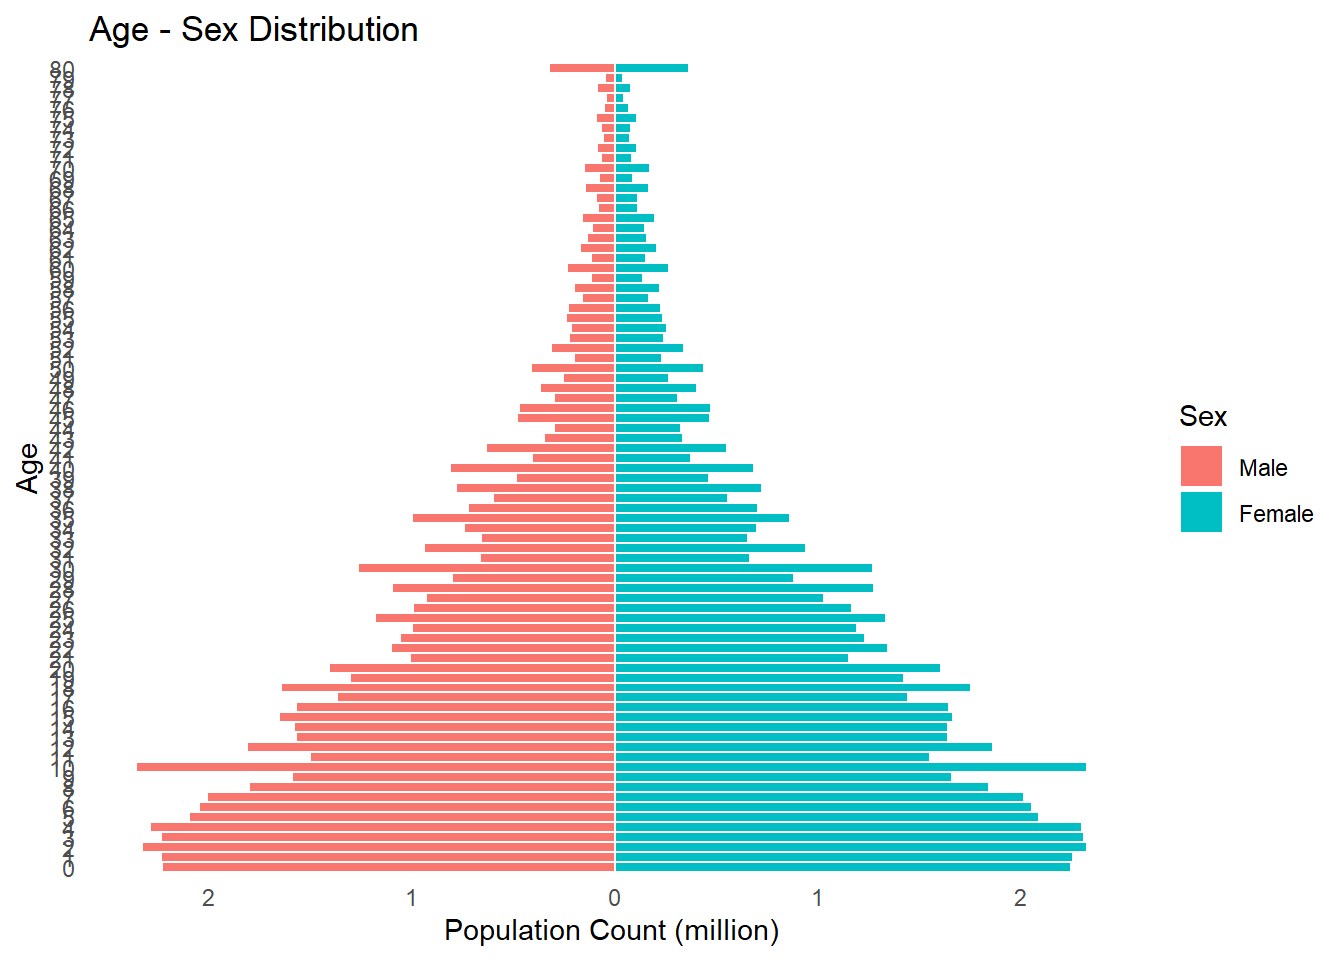
\includegraphics{indicators_notebook_files/figure-latex/unnamed-chunk-4-2.pdf}

\begin{itemize}
\tightlist
\item
  \emph{P42\_LAST\_12\_MON\_P = Live births in the past 12 months}
\end{itemize}

\begin{Shaded}
\begin{Highlighting}[]
\CommentTok{\# Unique values}
\NormalTok{demographics}\SpecialCharTok{$}\NormalTok{P42\_LAST\_12\_MON\_P }\SpecialCharTok{|\textgreater{}} \FunctionTok{str}\NormalTok{()}
\end{Highlighting}
\end{Shaded}

\begin{verbatim}
##  dbl+lbl [1:1321973]  2,  2,  2,  2, NA,  2,  2, NA,  2,  2,  2,  2, NA, NA...
##  @ label        : chr "Any live births in last 12 months?"
##  @ format.spss  : chr "F1.0"
##  @ display_width: int 19
##  @ labels       : Named num [1:2] 1 2
##   ..- attr(*, "names")= chr [1:2] "Yes" "No"
\end{verbatim}

\begin{Shaded}
\begin{Highlighting}[]
\CommentTok{\# distribution of live births in females}
\NormalTok{demographics }\SpecialCharTok{|\textgreater{}}
\NormalTok{  dplyr}\SpecialCharTok{::}\FunctionTok{filter}\NormalTok{(P4\_SEX\_P }\SpecialCharTok{==} \DecValTok{2}\NormalTok{) }\SpecialCharTok{|\textgreater{}}
  \FunctionTok{mutate}\NormalTok{(}\AttributeTok{P42\_LAST\_12\_MON\_P =} \FunctionTok{as\_factor}\NormalTok{(P42\_LAST\_12\_MON\_P)) }\SpecialCharTok{|\textgreater{}}
\NormalTok{  dplyr}\SpecialCharTok{::}\FunctionTok{group\_by}\NormalTok{(P42\_LAST\_12\_MON\_P) }\SpecialCharTok{|\textgreater{}}
  \FunctionTok{count}\NormalTok{(}\AttributeTok{name =} \StringTok{"Freq"}\NormalTok{) }\SpecialCharTok{|\textgreater{}}
\NormalTok{  tibble}\SpecialCharTok{::}\FunctionTok{tibble}\NormalTok{() }\SpecialCharTok{|\textgreater{}}
\NormalTok{  ggplot2}\SpecialCharTok{::}\FunctionTok{ggplot}\NormalTok{() }\SpecialCharTok{+}
\NormalTok{  ggplot2}\SpecialCharTok{::}\FunctionTok{geom\_bar}\NormalTok{(}\FunctionTok{aes}\NormalTok{(}\AttributeTok{x =}\NormalTok{ P42\_LAST\_12\_MON\_P , }\AttributeTok{fill =}\NormalTok{ P42\_LAST\_12\_MON\_P, }\AttributeTok{y =}\NormalTok{ Freq), }
                    \AttributeTok{stat =} \StringTok{"identity"}\NormalTok{) }\SpecialCharTok{+}
\NormalTok{  ggplot2}\SpecialCharTok{::}\FunctionTok{labs}\NormalTok{(}\AttributeTok{title =} \StringTok{"Distribution of Live Births in the past 12 Months"}\NormalTok{) }\SpecialCharTok{+}
\NormalTok{  ggplot2}\SpecialCharTok{::}\FunctionTok{theme\_minimal}\NormalTok{() }\SpecialCharTok{+}
\NormalTok{  ggplot2}\SpecialCharTok{::}\FunctionTok{theme}\NormalTok{(}
    \AttributeTok{plot.title =} \FunctionTok{element\_text}\NormalTok{(}\AttributeTok{hjust =} \FloatTok{0.5}\NormalTok{)}
\NormalTok{  )}
\end{Highlighting}
\end{Shaded}

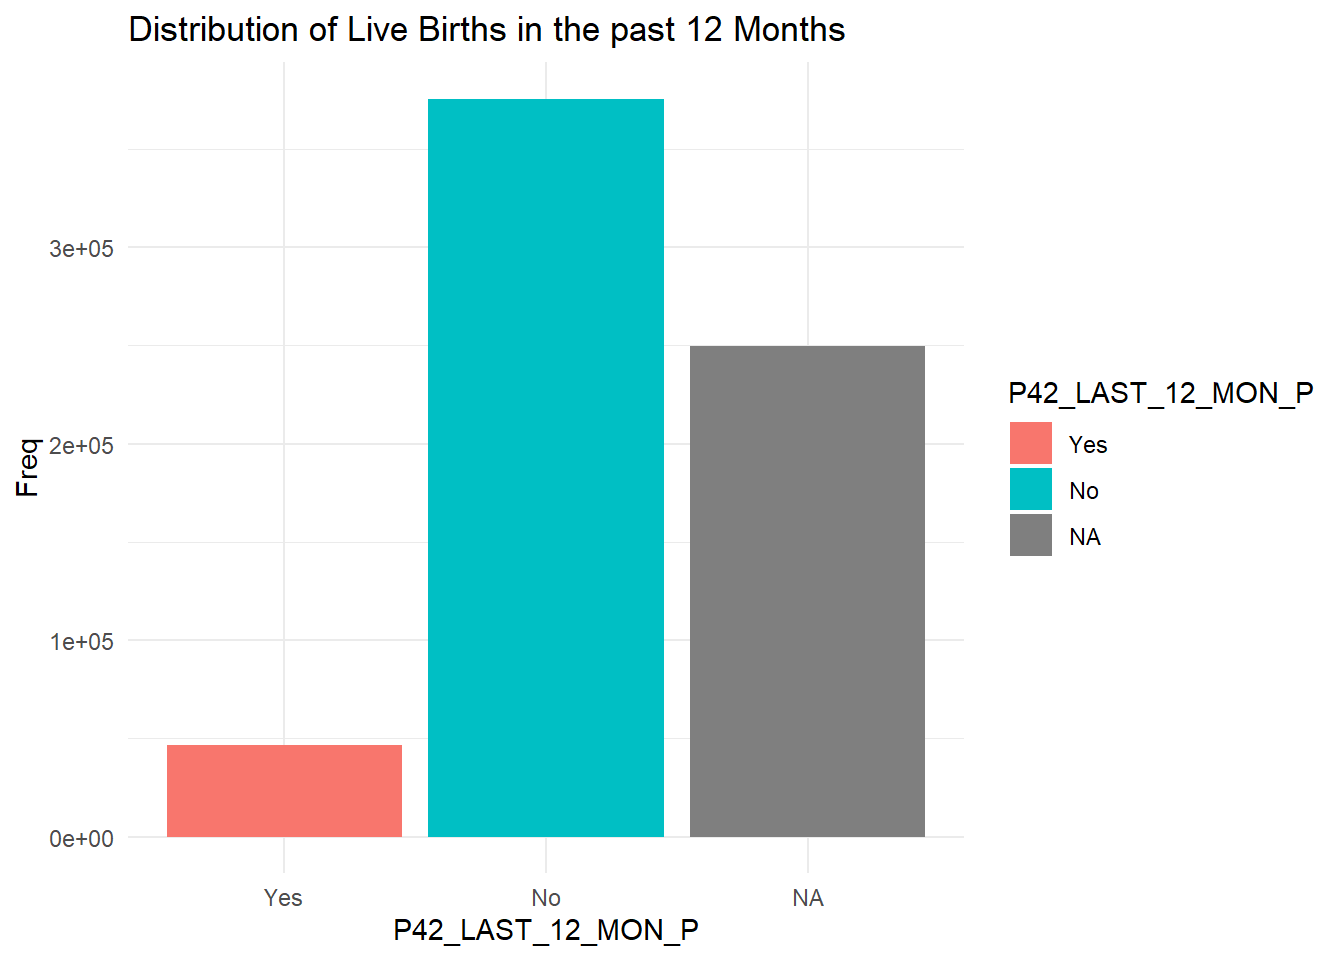
\includegraphics{indicators_notebook_files/figure-latex/unnamed-chunk-5-1.pdf}

\begin{itemize}
\tightlist
\item
  \emph{P32\_ACTIVITY\_LAST\_12\_MONTHS\_P = Activity in the last 12
  months}
\end{itemize}

\begin{Shaded}
\begin{Highlighting}[]
\CommentTok{\# Unique Activities}
\NormalTok{demographics}\SpecialCharTok{$}\NormalTok{P32\_ACTIVITY\_LAST\_12\_MONTHS\_P }\SpecialCharTok{|\textgreater{}} \FunctionTok{unique}\NormalTok{()}
\end{Highlighting}
\end{Shaded}

\begin{verbatim}
## <labelled<double>[12]>: Activity last twelve months
##  [1] NA  7 10  2  8  9  4  6 11  3  1  5
## 
## Labels:
##  value                                        label
##      1                   Worked - Paid non seasonal
##      2                 Worked - Unpaid non seasonal
##      3                       Worked - Paid seasonal
##      4                     Worked - Unpaid seasonal
##      5                                     On Leave
##      6 Unpaid work on household holding or business
##      7                  Unemployed and seeking work
##      8       Not seeking work but availabe for work
##      9                Full time housewife/homemaker
##     10                            Full time student
##     11     Not available for work for other reasons
\end{verbatim}

\begin{Shaded}
\begin{Highlighting}[]
\CommentTok{\# activity distribution}
\NormalTok{demographics }\SpecialCharTok{|\textgreater{}}
  \FunctionTok{mutate}\NormalTok{(}\AttributeTok{P32\_ACTIVITY\_LAST\_12\_MONTHS\_P =} \FunctionTok{as\_factor}\NormalTok{(P32\_ACTIVITY\_LAST\_12\_MONTHS\_P),}
         \AttributeTok{P4\_SEX\_P =} \FunctionTok{as\_factor}\NormalTok{(P4\_SEX\_P)}
\NormalTok{         ) }\SpecialCharTok{|\textgreater{}}
\NormalTok{  dplyr}\SpecialCharTok{::}\FunctionTok{group\_by}\NormalTok{(P32\_ACTIVITY\_LAST\_12\_MONTHS\_P, P4\_SEX\_P) }\SpecialCharTok{|\textgreater{}}
  \FunctionTok{count}\NormalTok{(}\AttributeTok{name =} \StringTok{"Freq"}\NormalTok{) }\SpecialCharTok{|\textgreater{}}
\NormalTok{  ggplot2}\SpecialCharTok{::}\FunctionTok{ggplot}\NormalTok{() }\SpecialCharTok{+}
\NormalTok{  ggplot2}\SpecialCharTok{::}\FunctionTok{geom\_bar}\NormalTok{(}\FunctionTok{aes}\NormalTok{(}\AttributeTok{y =}\NormalTok{ P32\_ACTIVITY\_LAST\_12\_MONTHS\_P, }
                        \AttributeTok{fill =}\NormalTok{ P4\_SEX\_P, }
                        \AttributeTok{x =}\NormalTok{ Freq), }
                    \AttributeTok{stat =} \StringTok{"identity"}\NormalTok{) }\SpecialCharTok{+}
\NormalTok{  ggplot2}\SpecialCharTok{::}\FunctionTok{theme\_minimal}\NormalTok{() }\SpecialCharTok{+}
\NormalTok{  ggplot2}\SpecialCharTok{::}\FunctionTok{theme}\NormalTok{(}
    \AttributeTok{panel.grid =} \FunctionTok{element\_blank}\NormalTok{(),}
    \AttributeTok{plot.title =} \FunctionTok{element\_text}\NormalTok{(}\AttributeTok{face =} \StringTok{"bold"}\NormalTok{)}
\NormalTok{  ) }\SpecialCharTok{+}
\NormalTok{  ggplot2}\SpecialCharTok{::}\FunctionTok{labs}\NormalTok{(}
    \AttributeTok{title =} \StringTok{"Frequency of Activities in the past 12 month by Sex"}\NormalTok{,}
    \AttributeTok{y =} \StringTok{"Activity"}
\NormalTok{  )}
\end{Highlighting}
\end{Shaded}

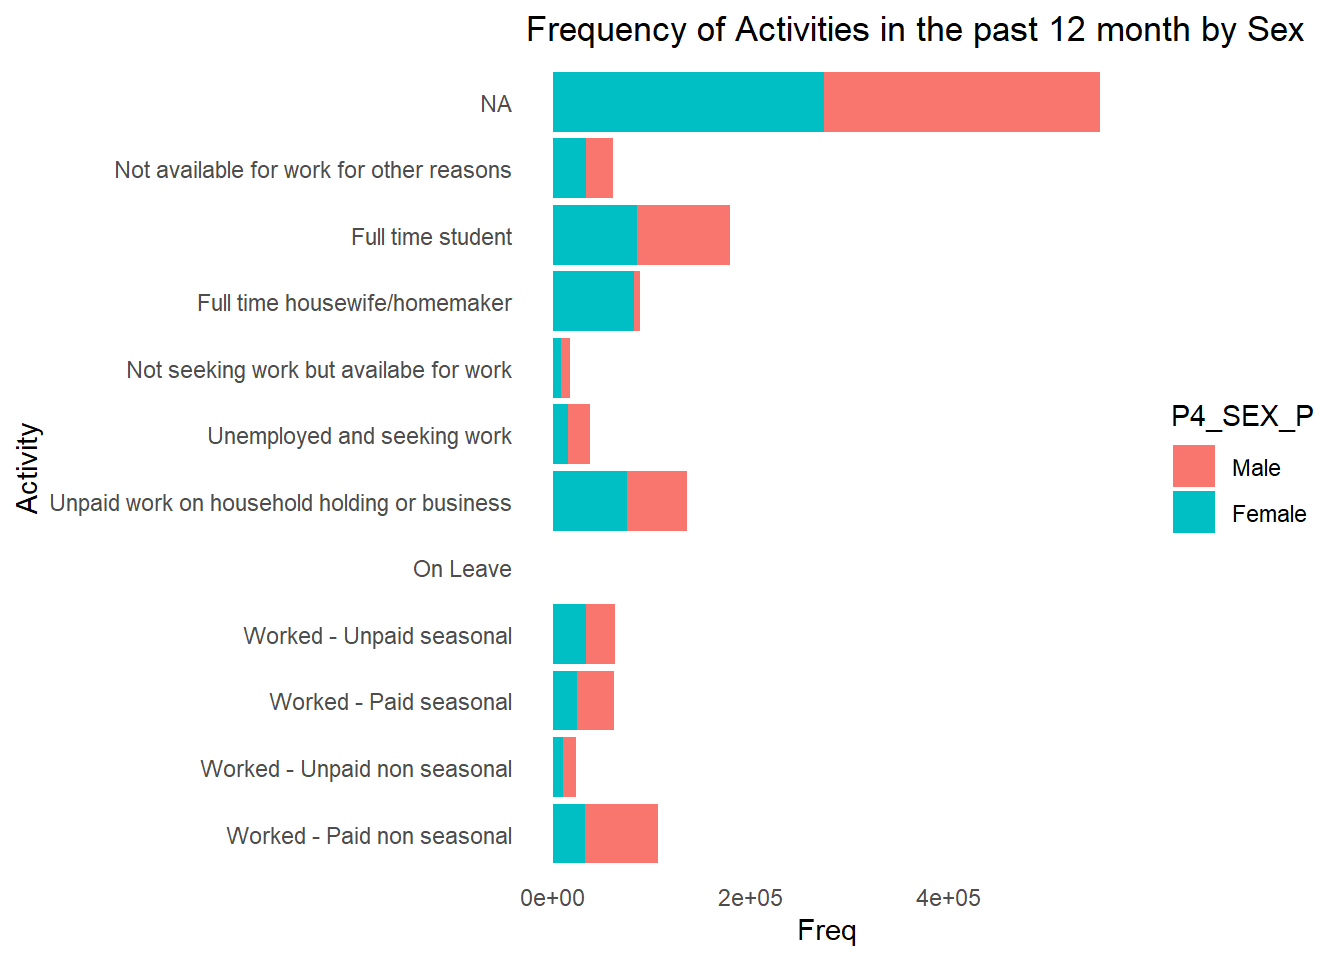
\includegraphics{indicators_notebook_files/figure-latex/unnamed-chunk-6-1.pdf}

\begin{itemize}
\tightlist
\item
  \emph{CONST\_P = Constituency (Admin 4)}
\end{itemize}

\begin{Shaded}
\begin{Highlighting}[]
\NormalTok{constituency\_shape }\SpecialCharTok{|\textgreater{}}
\NormalTok{  ggplot2}\SpecialCharTok{::}\FunctionTok{ggplot}\NormalTok{() }\SpecialCharTok{+}
\NormalTok{  ggplot2}\SpecialCharTok{::}\FunctionTok{geom\_sf}\NormalTok{(}\AttributeTok{color =} \StringTok{"black"}\NormalTok{) }\SpecialCharTok{+}
\NormalTok{  ggplot2}\SpecialCharTok{::}\FunctionTok{labs}\NormalTok{(}\AttributeTok{title =} \StringTok{"Zambia Constituencies 2010"}\NormalTok{) }\SpecialCharTok{+}
\NormalTok{  ggplot2}\SpecialCharTok{::}\FunctionTok{theme\_void}\NormalTok{() }\SpecialCharTok{+}
\NormalTok{  ggplot2}\SpecialCharTok{::}\FunctionTok{theme}\NormalTok{(}
    \AttributeTok{plot.title =} \FunctionTok{element\_text}\NormalTok{(}\AttributeTok{hjust =} \FloatTok{0.5}\NormalTok{, }\AttributeTok{face =} \StringTok{"bold"}\NormalTok{)}
\NormalTok{  )}
\end{Highlighting}
\end{Shaded}

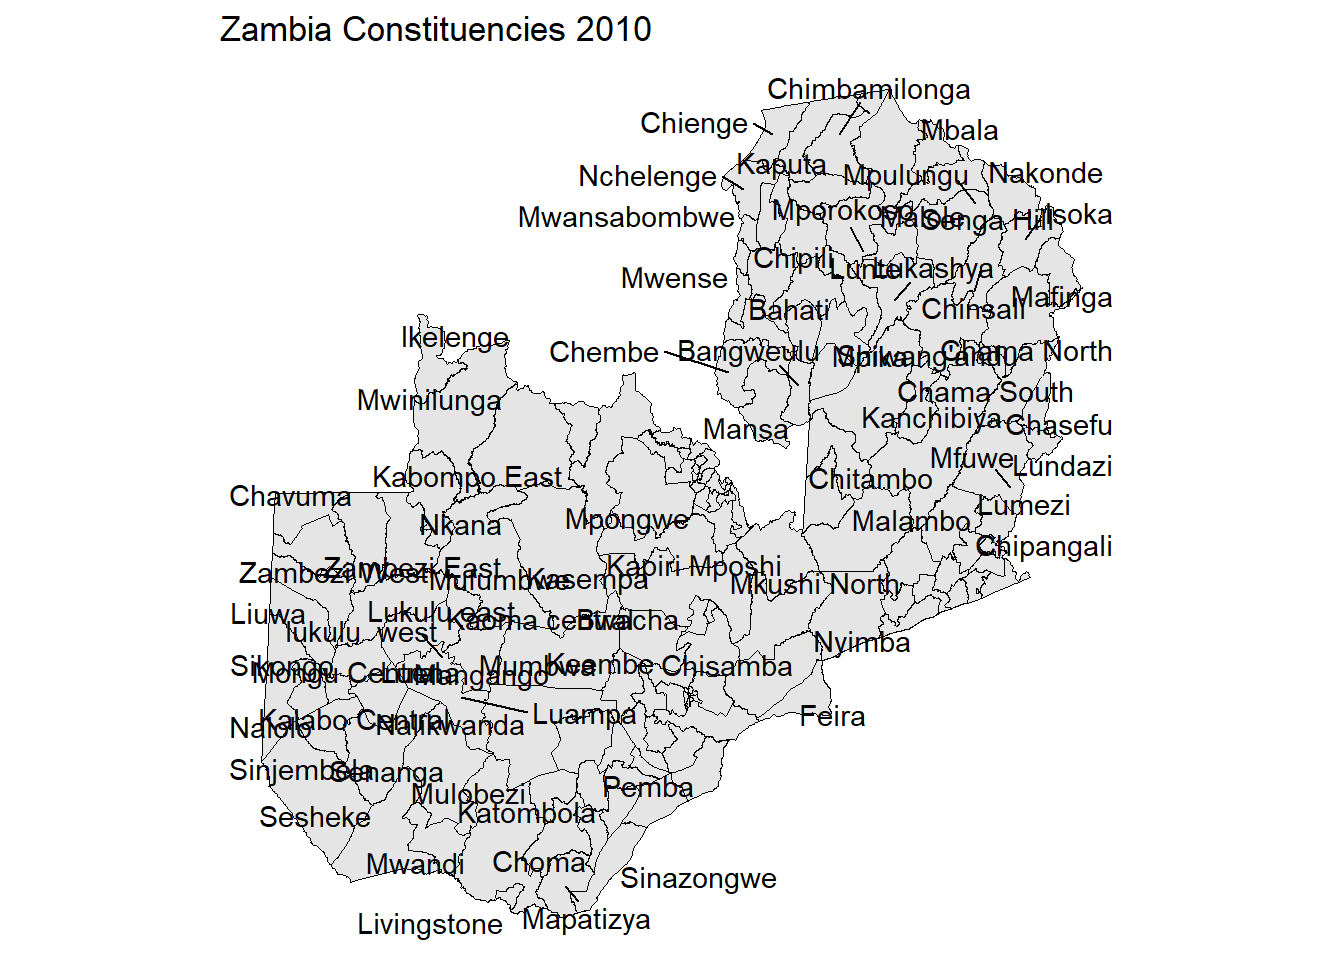
\includegraphics{indicators_notebook_files/figure-latex/unnamed-chunk-7-1.pdf}

\subsection{SUSTAINABLE DEVELOPMENT GOALS (SDG)
CALCULATION}\label{sustainable-development-goals-sdg-calculation}

\subsubsection{SDG 3 : Good Health and Well
Being}\label{sdg-3-good-health-and-well-being}

\paragraph{SDG TARGET 3.7: By 2030, ensure universal access to sexual
and reproductive health-care services, including for family planning,
information and education, and the integration of reproductive health
into national strategies and
programmes.}\label{sdg-target-3.7-by-2030-ensure-universal-access-to-sexual-and-reproductive-health-care-services-including-for-family-planning-information-and-education-and-the-integration-of-reproductive-health-into-national-strategies-and-programmes.}

\subparagraph{\texorpdfstring{\textbf{SDG Indicator 3.7.2: Adolescent
birth rate (aged 10--14 years; aged 15--19 years) per 1,000 women in
that age
group}}{SDG Indicator 3.7.2: Adolescent birth rate (aged 10--14 years; aged 15--19 years) per 1,000 women in that age group}}\label{sdg-indicator-3.7.2-adolescent-birth-rate-aged-1014-years-aged-1519-years-per-1000-women-in-that-age-group}

The adolescent birth rate for 10--14 years is calculated as

\(\text{Adolescent Birth Rate}_{10-14} = \left( \frac{\text{Number of women aged 10-14 with live birth in the past 12 months}}{\text{Number of women aged 10-14}} \right) \times 1000\)

and for 15--19 years as

\(\text{Adolescent Birth Rate}_{15-19} = \left( \frac{\text{Number of women aged 15-19 with live birth in the past 12 months}}{\text{Number of women aged 15-19}} \right) \times 1000\)

\textbf{Input Variables Definition:}

\begin{itemize}
\item
  \emph{P4\_SEX\_P = Sex}
\item
  \emph{P5\_AGE\_P = Age}
\item
  \emph{P42\_LAST\_12\_MON\_P = Live births in the past 12 months}
\item
  \emph{CONST\_P = Constituency (Admin 4)}
\end{itemize}

\textbf{Output Variables Definition:}

\begin{itemize}
\item
  \emph{total.ado.10\_14 = Total female adolescents aged 10 to 14}
\item
  \emph{total.ado.15\_19 = Total female adolescents aged 15 to 19}
\item
  \emph{total.ado.birth.10\_14 = Total female adolescents aged 10 to 14
  with live birth in the past 12 months}
\item
  \emph{total.ado.birth.15\_19 = Total female adolescents aged 15 to 19
  with live birth in the past 12 months}
\item
  \emph{abr.10\_14 = Adolescent aged 10 to 14 birth rate}
\item
  \emph{abr.15\_19 = Adolescent aged 15 to 19 birth rate}
\end{itemize}

\textbf{Methodology:}

1- Filter the Sex to Female by using the P4\_SEX\_P == 2

2- Group by the constituency

3- Compute summary statistics

\textbf{Adolescent Birth Rate by Constituency}

\begin{Shaded}
\begin{Highlighting}[]
\NormalTok{adolescent\_birth\_rate }\OtherTok{\textless{}{-}} 
\NormalTok{  demographics }\SpecialCharTok{|\textgreater{}}
\NormalTok{  dplyr}\SpecialCharTok{::}\FunctionTok{filter}\NormalTok{(P4\_SEX\_P }\SpecialCharTok{==} \DecValTok{2}\NormalTok{) }\SpecialCharTok{|\textgreater{}}
\NormalTok{  dplyr}\SpecialCharTok{::}\FunctionTok{group\_by}\NormalTok{(CONST\_P) }\SpecialCharTok{|\textgreater{}}
\NormalTok{  dplyr}\SpecialCharTok{::}\FunctionTok{summarise}\NormalTok{(}
    \AttributeTok{total.ado.10\_14 =} \FunctionTok{sum}\NormalTok{(dplyr}\SpecialCharTok{::}\FunctionTok{between}\NormalTok{(P5\_AGE\_P, }\DecValTok{10}\NormalTok{, }\DecValTok{14}\NormalTok{), }\AttributeTok{na.rm =} \ConstantTok{TRUE}\NormalTok{),}
    \AttributeTok{total.ado.15\_19 =} \FunctionTok{sum}\NormalTok{(dplyr}\SpecialCharTok{::}\FunctionTok{between}\NormalTok{(P5\_AGE\_P, }\DecValTok{15}\NormalTok{, }\DecValTok{19}\NormalTok{), }\AttributeTok{na.rm =} \ConstantTok{TRUE}\NormalTok{),}
    \AttributeTok{total.ado.birth.10\_14 =} \FunctionTok{sum}\NormalTok{(dplyr}\SpecialCharTok{::}\FunctionTok{between}\NormalTok{(P5\_AGE\_P, }\DecValTok{10}\NormalTok{, }\DecValTok{14}\NormalTok{) }\SpecialCharTok{\&}
\NormalTok{                                  P42\_LAST\_12\_MON\_P }\SpecialCharTok{==} \DecValTok{1}\NormalTok{, }\AttributeTok{na.rm =} \ConstantTok{TRUE}\NormalTok{),}
    \AttributeTok{total.ado.birth.15\_19 =} \FunctionTok{sum}\NormalTok{(dplyr}\SpecialCharTok{::}\FunctionTok{between}\NormalTok{(P5\_AGE\_P, }\DecValTok{15}\NormalTok{, }\DecValTok{19}\NormalTok{) }\SpecialCharTok{\&}
\NormalTok{                                  P42\_LAST\_12\_MON\_P }\SpecialCharTok{==} \DecValTok{1}\NormalTok{, }\AttributeTok{na.rm =} \ConstantTok{TRUE}\NormalTok{),}
    \AttributeTok{abr.10\_14 =} \FunctionTok{round}\NormalTok{((total.ado.birth}\FloatTok{.10}\NormalTok{\_14 }\SpecialCharTok{/}\NormalTok{ total.ado}\FloatTok{.10}\NormalTok{\_14) }\SpecialCharTok{*} \DecValTok{1000}\NormalTok{,}\DecValTok{2}\NormalTok{),}
    \AttributeTok{abr.15\_19 =} \FunctionTok{round}\NormalTok{((total.ado.birth}\FloatTok{.15}\NormalTok{\_19 }\SpecialCharTok{/}\NormalTok{ total.ado}\FloatTok{.15}\NormalTok{\_19) }\SpecialCharTok{*} \DecValTok{1000}\NormalTok{,}\DecValTok{2}\NormalTok{)}
\NormalTok{  ) }\SpecialCharTok{|\textgreater{}}
\NormalTok{  dplyr}\SpecialCharTok{::}\FunctionTok{mutate}\NormalTok{(}
    \AttributeTok{CONST\_P\_name =}\NormalTok{ forcats}\SpecialCharTok{::}\FunctionTok{as\_factor}\NormalTok{(CONST\_P)}
\NormalTok{  ) }\SpecialCharTok{|\textgreater{}}
\NormalTok{  dplyr}\SpecialCharTok{::}\FunctionTok{select}\NormalTok{(}
\NormalTok{    CONST\_P\_name,}
    \FunctionTok{everything}\NormalTok{()}
\NormalTok{  ) }

\CommentTok{\# Print table}
\NormalTok{adolescent\_birth\_rate }\SpecialCharTok{|\textgreater{}}
  \FunctionTok{head}\NormalTok{() }\SpecialCharTok{|\textgreater{}}
\NormalTok{  gt}\SpecialCharTok{::}\FunctionTok{gt}\NormalTok{()}
\end{Highlighting}
\end{Shaded}

\begin{table}[!t]
\fontsize{12.0pt}{14.4pt}\selectfont
\begin{tabular*}{\linewidth}{@{\extracolsep{\fill}}ccrrrrrr}
\toprule
Constituency & Constituency & total.ado.10\_14 & total.ado.15\_19 & total.ado.birth.10\_14 & total.ado.birth.15\_19 & abr.10\_14 & abr.15\_19 \\ 
\midrule\addlinespace[2.5pt]
Chisamba & 1 & 753 & 622 & 2 & 60 & 2.66 & 96.46 \\ 
Katuba & 2 & 613 & 523 & 0 & 39 & 0.00 & 74.57 \\ 
Keembe & 3 & 883 & 740 & 4 & 75 & 4.53 & 101.35 \\ 
Bwacha & 4 & 588 & 559 & 0 & 31 & 0.00 & 55.46 \\ 
Kabwe Central & 5 & 881 & 950 & 6 & 52 & 6.81 & 54.74 \\ 
Kapiri Mposhi & 6 & 1828 & 1507 & 2 & 140 & 1.09 & 92.90 \\ 
\bottomrule
\end{tabular*}
\end{table}

\textbf{Visualization}

\begin{Shaded}
\begin{Highlighting}[]
\NormalTok{constituency\_shape }\SpecialCharTok{|\textgreater{}}
\NormalTok{  dplyr}\SpecialCharTok{::}\FunctionTok{select}\NormalTok{(NAME1\_, geometry) }\SpecialCharTok{|\textgreater{}}
\NormalTok{  dplyr}\SpecialCharTok{::}\FunctionTok{left\_join}\NormalTok{(}
\NormalTok{    adolescent\_birth\_rate,}
    \AttributeTok{by =} \FunctionTok{c}\NormalTok{(}\StringTok{"NAME1\_"} \OtherTok{=} \StringTok{"CONST\_P\_name"}\NormalTok{)}
\NormalTok{  ) }\SpecialCharTok{|\textgreater{}}
\NormalTok{  tidyr}\SpecialCharTok{::}\FunctionTok{pivot\_longer}\NormalTok{(}
    \AttributeTok{cols =} \FunctionTok{c}\NormalTok{(}\StringTok{"abr.10\_14"}\NormalTok{, }\StringTok{"abr.15\_19"}\NormalTok{),}
    \AttributeTok{names\_to =} \StringTok{"abr\_cat"}\NormalTok{,}
    \AttributeTok{values\_to =} \StringTok{"abr\_rate"}
\NormalTok{  ) }\SpecialCharTok{|\textgreater{}}
\NormalTok{  ggplot2}\SpecialCharTok{::}\FunctionTok{ggplot}\NormalTok{() }\SpecialCharTok{+}
\NormalTok{  ggplot2}\SpecialCharTok{::}\FunctionTok{geom\_sf}\NormalTok{(}\FunctionTok{aes}\NormalTok{(}\AttributeTok{fill =}\NormalTok{ abr\_rate), }\AttributeTok{color =} \StringTok{"white"}\NormalTok{) }\SpecialCharTok{+}
\NormalTok{  ggplot2}\SpecialCharTok{::}\FunctionTok{scale\_fill\_distiller}\NormalTok{(}\AttributeTok{palette =} \StringTok{"RdPu"}\NormalTok{, }\AttributeTok{direction =} \DecValTok{1}\NormalTok{) }\SpecialCharTok{+}
\NormalTok{  ggplot2}\SpecialCharTok{::}\FunctionTok{theme\_void}\NormalTok{() }\SpecialCharTok{+}
\NormalTok{  ggplot2}\SpecialCharTok{::}\FunctionTok{labs}\NormalTok{(}\AttributeTok{title =} \StringTok{"Adolescent Birth Rate per 1000"}\NormalTok{) }\SpecialCharTok{+}
\NormalTok{  ggplot2}\SpecialCharTok{::}\FunctionTok{theme}\NormalTok{(}
    \AttributeTok{legend.position =} \StringTok{"bottom"}\NormalTok{,}
    \AttributeTok{plot.title =} \FunctionTok{element\_text}\NormalTok{(}\AttributeTok{hjust =} \FloatTok{0.5}\NormalTok{, }\AttributeTok{face =} \StringTok{"bold"}\NormalTok{)}
\NormalTok{  ) }\SpecialCharTok{+}
\NormalTok{  ggplot2}\SpecialCharTok{::}\FunctionTok{facet\_grid}\NormalTok{(}\SpecialCharTok{\textasciitilde{}}\NormalTok{abr\_cat)}
\end{Highlighting}
\end{Shaded}

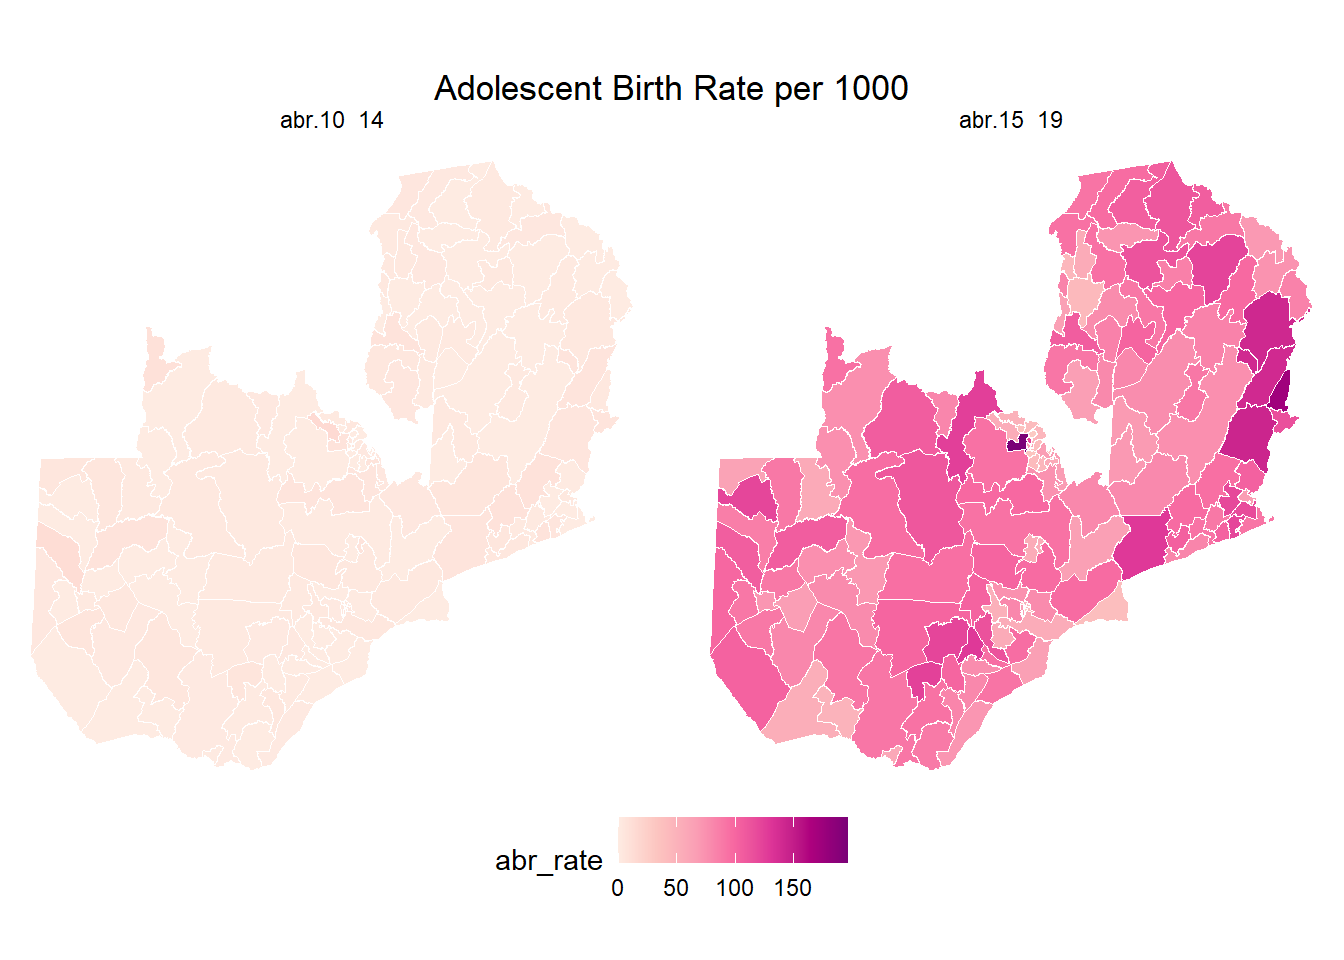
\includegraphics{indicators_notebook_files/figure-latex/unnamed-chunk-9-1.pdf}

\subsubsection{SDG 5 : GENDER EQUALITY}\label{sdg-5-gender-equality}

\paragraph{SDG TARGET 5.3 : Eliminate all harmful practices, such as
child, early and forced marriage and female genital
mutilations}\label{sdg-target-5.3-eliminate-all-harmful-practices-such-as-child-early-and-forced-marriage-and-female-genital-mutilations}

\subparagraph{\texorpdfstring{\textbf{SDG INDICATOR 5.3.1: Proportion of
women aged 20--24 years who were married or in a union before age 15 and
before age
18}}{SDG INDICATOR 5.3.1: Proportion of women aged 20--24 years who were married or in a union before age 15 and before age 18}}\label{sdg-indicator-5.3.1-proportion-of-women-aged-2024-years-who-were-married-or-in-a-union-before-age-15-and-before-age-18}

The child marriage indicator before age 15 is calculated as

\(\text{Child Marriage Before Age 15} = \left( \frac{\text{Number of women aged 20–24 married before age 15}}{\text{Total number of women aged 20–24}} \right) \times 100\)

and before age 18 as

\(\text{Child Marriage Before Age 18} = \left( \frac{\text{Number of women aged 20–24 married before age 18}}{\text{Total number of women aged 20–24}} \right) \times 100\)

\textbf{Input Variables Definition:}

\begin{itemize}
\item
  \emph{P4\_SEX\_P = Sex (1 - Male, 2 - Female)}
\item
  \emph{P5\_AGE\_P = Age}
\item
  \emph{CONST\_P = Constituency}
\end{itemize}

\textbf{Output Variable Definition:}

\begin{itemize}
\item
  \emph{total.girls.20\_24 = Total number of females aged 20 to 24}
\item
  \emph{married.before.15 = Total number of females married before 15}
\item
  \emph{married.before.18 = Total number of females married before 18}
\item
  \emph{prop.cm.before.15 = Proportion of child marriages before 15}
\item
  \emph{prop.cm.before.18 = Proportion of child marriages before 18}
\end{itemize}

\textbf{\emph{Child Marriage by Constituency (Admin 4 Zambia)}}

\begin{Shaded}
\begin{Highlighting}[]
\NormalTok{child\_marriage }\OtherTok{\textless{}{-}} 
\NormalTok{  demographics }\SpecialCharTok{|\textgreater{}}
\NormalTok{  dplyr}\SpecialCharTok{::}\FunctionTok{filter}\NormalTok{(P5\_AGE\_P }\SpecialCharTok{\textgreater{}=} \DecValTok{20}\NormalTok{, P5\_AGE\_P }\SpecialCharTok{\textless{}=} \DecValTok{24}\NormalTok{, P4\_SEX\_P }\SpecialCharTok{==} \DecValTok{2}\NormalTok{) }\SpecialCharTok{|\textgreater{}}
\NormalTok{  dplyr}\SpecialCharTok{::}\FunctionTok{group\_by}\NormalTok{(CONST\_P) }\SpecialCharTok{|\textgreater{}}
\NormalTok{  dplyr}\SpecialCharTok{::}\FunctionTok{summarise}\NormalTok{(}
    \AttributeTok{total.girls.20\_24 =} \FunctionTok{n}\NormalTok{(),}
    \AttributeTok{married.before.15 =} \FunctionTok{sum}\NormalTok{(P37\_AGE\_FIRST\_MARRAIGE\_P }\SpecialCharTok{\textless{}} \DecValTok{15}\NormalTok{, }\AttributeTok{na.rm =}\NormalTok{ T),}
    \AttributeTok{married.before.18 =} \FunctionTok{sum}\NormalTok{(P37\_AGE\_FIRST\_MARRAIGE\_P }\SpecialCharTok{\textless{}} \DecValTok{18}\NormalTok{, }\AttributeTok{na.rm =}\NormalTok{ T),}
    \AttributeTok{prop.cm.before.15 =} \FunctionTok{round}\NormalTok{(married.before}\FloatTok{.15} \SpecialCharTok{/}\NormalTok{ total.girls}\FloatTok{.20}\NormalTok{\_24, }\DecValTok{2}\NormalTok{),}
    \AttributeTok{prop.cm.before.18 =} \FunctionTok{round}\NormalTok{(married.before}\FloatTok{.18} \SpecialCharTok{/}\NormalTok{ total.girls}\FloatTok{.20}\NormalTok{\_24, }\DecValTok{2}\NormalTok{)}
\NormalTok{  ) }\SpecialCharTok{|\textgreater{}}
\NormalTok{  dplyr}\SpecialCharTok{::}\FunctionTok{mutate}\NormalTok{(}
    \AttributeTok{CONST\_P\_name =}\NormalTok{ forcats}\SpecialCharTok{::}\FunctionTok{as\_factor}\NormalTok{(CONST\_P)}
\NormalTok{  ) }\SpecialCharTok{|\textgreater{}}
\NormalTok{  dplyr}\SpecialCharTok{::}\FunctionTok{select}\NormalTok{(}
\NormalTok{    CONST\_P\_name,}
    \FunctionTok{everything}\NormalTok{()}
\NormalTok{  )}

\CommentTok{\# print table}
\NormalTok{child\_marriage }\SpecialCharTok{|\textgreater{}}
  \FunctionTok{head}\NormalTok{() }\SpecialCharTok{|\textgreater{}}
\NormalTok{  gt}\SpecialCharTok{::}\FunctionTok{gt}\NormalTok{()}
\end{Highlighting}
\end{Shaded}

\begin{table}[!t]
\fontsize{12.0pt}{14.4pt}\selectfont
\begin{tabular*}{\linewidth}{@{\extracolsep{\fill}}ccrrrrr}
\toprule
Constituency & Constituency & total.girls.20\_24 & married.before.15 & married.before.18 & prop.cm.before.15 & prop.cm.before.18 \\ 
\midrule\addlinespace[2.5pt]
Chisamba & 1 & 459 & 9 & 112 & 0.02 & 0.24 \\ 
Katuba & 2 & 376 & 13 & 101 & 0.03 & 0.27 \\ 
Keembe & 3 & 567 & 29 & 176 & 0.05 & 0.31 \\ 
Bwacha & 4 & 414 & 15 & 91 & 0.04 & 0.22 \\ 
Kabwe Central & 5 & 716 & 8 & 85 & 0.01 & 0.12 \\ 
Kapiri Mposhi & 6 & 1153 & 57 & 344 & 0.05 & 0.30 \\ 
\bottomrule
\end{tabular*}
\end{table}

\textbf{Visualization}

\begin{Shaded}
\begin{Highlighting}[]
\NormalTok{constituency\_shape }\SpecialCharTok{|\textgreater{}}
\NormalTok{  dplyr}\SpecialCharTok{::}\FunctionTok{select}\NormalTok{(NAME1\_, geometry) }\SpecialCharTok{|\textgreater{}}
\NormalTok{  dplyr}\SpecialCharTok{::}\FunctionTok{left\_join}\NormalTok{(}
\NormalTok{    child\_marriage,}
    \AttributeTok{by =} \FunctionTok{c}\NormalTok{(}\StringTok{"NAME1\_"} \OtherTok{=} \StringTok{"CONST\_P\_name"}\NormalTok{)}
\NormalTok{  ) }\SpecialCharTok{|\textgreater{}}
\NormalTok{  tidyr}\SpecialCharTok{::}\FunctionTok{pivot\_longer}\NormalTok{(}
    \AttributeTok{cols =} \FunctionTok{c}\NormalTok{(}\StringTok{"prop.cm.before.15"}\NormalTok{, }\StringTok{"prop.cm.before.18"}\NormalTok{),}
    \AttributeTok{names\_to =} \StringTok{"child\_marriage"}\NormalTok{,}
    \AttributeTok{values\_to =} \StringTok{"cm\_rate"}
\NormalTok{  ) }\SpecialCharTok{|\textgreater{}}
\NormalTok{  ggplot2}\SpecialCharTok{::}\FunctionTok{ggplot}\NormalTok{() }\SpecialCharTok{+}
\NormalTok{  ggplot2}\SpecialCharTok{::}\FunctionTok{geom\_sf}\NormalTok{(}\FunctionTok{aes}\NormalTok{(}\AttributeTok{fill =}\NormalTok{ cm\_rate), }\AttributeTok{color =} \StringTok{"white"}\NormalTok{) }\SpecialCharTok{+}
\NormalTok{  ggplot2}\SpecialCharTok{::}\FunctionTok{scale\_fill\_distiller}\NormalTok{(}\AttributeTok{palette =} \StringTok{"RdPu"}\NormalTok{, }\AttributeTok{direction =} \DecValTok{1}\NormalTok{) }\SpecialCharTok{+}
\NormalTok{  ggplot2}\SpecialCharTok{::}\FunctionTok{theme\_void}\NormalTok{() }\SpecialCharTok{+}
\NormalTok{  ggplot2}\SpecialCharTok{::}\FunctionTok{labs}\NormalTok{(}\AttributeTok{title =} \StringTok{"Child Marriage"}\NormalTok{) }\SpecialCharTok{+}
\NormalTok{  ggplot2}\SpecialCharTok{::}\FunctionTok{theme}\NormalTok{(}
    \AttributeTok{legend.position =} \StringTok{"bottom"}\NormalTok{,}
    \AttributeTok{plot.title =} \FunctionTok{element\_text}\NormalTok{(}\AttributeTok{hjust =} \FloatTok{0.5}\NormalTok{, }\AttributeTok{face =} \StringTok{"bold"}\NormalTok{)}
\NormalTok{  ) }\SpecialCharTok{+}
\NormalTok{  ggplot2}\SpecialCharTok{::}\FunctionTok{facet\_grid}\NormalTok{(}\SpecialCharTok{\textasciitilde{}}\NormalTok{child\_marriage)}
\end{Highlighting}
\end{Shaded}

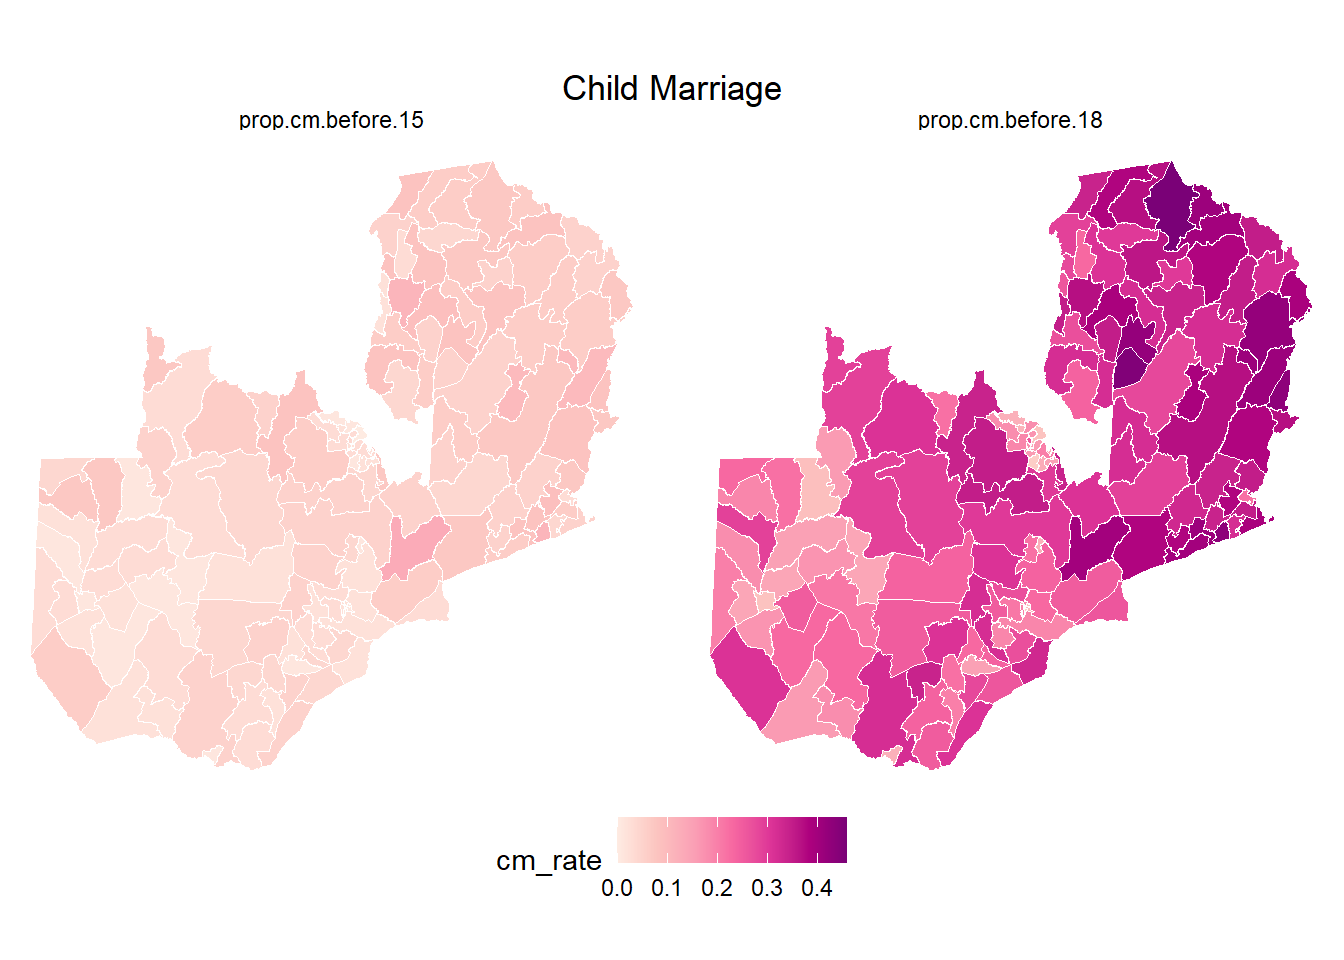
\includegraphics{indicators_notebook_files/figure-latex/unnamed-chunk-11-1.pdf}

\subsubsection{SDG 8 : DECENT WORK AND ECONOMIC
GROWTH}\label{sdg-8-decent-work-and-economic-growth}

\paragraph{SDG TARGET 8.6 : By 2020, substantially reduce the proportion
of youth not in employment, education or
training}\label{sdg-target-8.6-by-2020-substantially-reduce-the-proportion-of-youth-not-in-employment-education-or-training}

\subparagraph{\texorpdfstring{\textbf{SDG INDICATOR 8.6.1: Proportion of
youth (aged 15-24 years) not in education, employment or
training}}{SDG INDICATOR 8.6.1: Proportion of youth (aged 15-24 years) not in education, employment or training}}\label{sdg-indicator-8.6.1-proportion-of-youth-aged-15-24-years-not-in-education-employment-or-training}

The NEET rate is calculated as

\(\text{NEET Rate (%)} = \left( \frac{\text{Youth} - \text{Youth in employment} - \text{Youth not in employment but in education or training}}{\text{Youth}} \right) \times 100
\).

\textbf{Input Variables Definition :}

\begin{itemize}
\item
  \emph{P32\_ACTIVITY\_LAST\_12\_MONTHS\_P = Activity in the last 12
  months}
\item
  \emph{P5\_AGE\_P = Age}
\item
  \emph{CONST\_P = Constituency (Admin 4)}
\end{itemize}

\textbf{Output Variables Definition :}

\begin{itemize}
\item
  \emph{total.youth.15\_24 = Total number of people aged 15 to 24
  (Youth)}
\item
  \emph{total.neet = Number of youths not employed, not in education or
  training}
\item
  \emph{rate.need = proportion of youths not employed, not in education
  or training}
\end{itemize}

\textbf{\emph{Youth Unemployment by Constituency (Admin 4 Zambia) \&
Sex}}

\begin{Shaded}
\begin{Highlighting}[]
\NormalTok{youth\_umemplyment }\OtherTok{\textless{}{-}} 
\NormalTok{  demographics }\SpecialCharTok{|\textgreater{}}
\NormalTok{  dplyr}\SpecialCharTok{::}\FunctionTok{mutate}\NormalTok{(}
    \AttributeTok{Employ =} \FunctionTok{case\_when}\NormalTok{(}
\NormalTok{      P32\_ACTIVITY\_LAST\_12\_MONTHS\_P }\SpecialCharTok{\%in\%} \DecValTok{1}\SpecialCharTok{:}\DecValTok{6} \SpecialCharTok{\textasciitilde{}} \DecValTok{1}\NormalTok{,}
\NormalTok{      P32\_ACTIVITY\_LAST\_12\_MONTHS\_P }\SpecialCharTok{\%in\%} \DecValTok{7}\SpecialCharTok{:}\DecValTok{9} \SpecialCharTok{\textasciitilde{}} \DecValTok{2}\NormalTok{,}
\NormalTok{      P32\_ACTIVITY\_LAST\_12\_MONTHS\_P }\SpecialCharTok{==} \DecValTok{10} \SpecialCharTok{\textasciitilde{}} \DecValTok{3}\NormalTok{,}
\NormalTok{      T }\SpecialCharTok{\textasciitilde{}} \DecValTok{2}
\NormalTok{    )}
\NormalTok{  ) }\SpecialCharTok{|\textgreater{}}
\NormalTok{  dplyr}\SpecialCharTok{::}\FunctionTok{filter}\NormalTok{(P5\_AGE\_P }\SpecialCharTok{\textgreater{}=} \DecValTok{15}\NormalTok{, P5\_AGE\_P }\SpecialCharTok{\textless{}=} \DecValTok{24}\NormalTok{) }\SpecialCharTok{|\textgreater{}}
\NormalTok{  dplyr}\SpecialCharTok{::}\FunctionTok{group\_by}\NormalTok{(CONST\_P, P4\_SEX\_P) }\SpecialCharTok{|\textgreater{}}
  \FunctionTok{summarise}\NormalTok{(}
    \AttributeTok{total.youth.15\_24 =} \FunctionTok{n}\NormalTok{(),}
    \AttributeTok{total.neet =} \FunctionTok{sum}\NormalTok{(Employ }\SpecialCharTok{==} \DecValTok{2}\NormalTok{, }\AttributeTok{na.rm =} \ConstantTok{TRUE}\NormalTok{),}
    \AttributeTok{rate.neet =} \FunctionTok{round}\NormalTok{(total.neet }\SpecialCharTok{/}\NormalTok{ total.youth}\FloatTok{.15}\NormalTok{\_24, }\DecValTok{2}\NormalTok{)}
\NormalTok{  ) }\SpecialCharTok{|\textgreater{}}
\NormalTok{  dplyr}\SpecialCharTok{::}\FunctionTok{mutate}\NormalTok{(}
    \AttributeTok{CONST\_P\_name =}\NormalTok{ forcats}\SpecialCharTok{::}\FunctionTok{as\_factor}\NormalTok{(CONST\_P),}
    \AttributeTok{P4\_SEX\_P =}\NormalTok{ forcats}\SpecialCharTok{::}\FunctionTok{as\_factor}\NormalTok{(P4\_SEX\_P)}
\NormalTok{  ) }\SpecialCharTok{|\textgreater{}}
\NormalTok{  dplyr}\SpecialCharTok{::}\FunctionTok{select}\NormalTok{(}
\NormalTok{    CONST\_P\_name,}
    \FunctionTok{everything}\NormalTok{()}
\NormalTok{  ) }\SpecialCharTok{|\textgreater{}}
\NormalTok{  tidyr}\SpecialCharTok{::}\FunctionTok{pivot\_wider}\NormalTok{(}
    \AttributeTok{names\_from =}\NormalTok{  P4\_SEX\_P,}
    \AttributeTok{values\_from =} \DecValTok{4}\SpecialCharTok{:}\DecValTok{6}
\NormalTok{  ) }

\CommentTok{\# print table}
\NormalTok{youth\_umemplyment }\SpecialCharTok{|\textgreater{}}
\NormalTok{  tibble}\SpecialCharTok{::}\FunctionTok{tibble}\NormalTok{() }\SpecialCharTok{|\textgreater{}}
  \FunctionTok{head}\NormalTok{() }\SpecialCharTok{|\textgreater{}}
\NormalTok{  gt}\SpecialCharTok{::}\FunctionTok{gt}\NormalTok{()}
\end{Highlighting}
\end{Shaded}

\begin{table}[!t]
\fontsize{12.0pt}{14.4pt}\selectfont
\begin{tabular*}{\linewidth}{@{\extracolsep{\fill}}ccrrrrrr}
\toprule
CONST\_P\_name & Constituency & total.youth.15\_24\_Male & total.youth.15\_24\_Female & total.neet\_Male & total.neet\_Female & rate.neet\_Male & rate.neet\_Female \\ 
\midrule\addlinespace[2.5pt]
Chisamba & 1 & 1078 & 1081 & 300 & 478 & 0.28 & 0.44 \\ 
Katuba & 2 & 834 & 899 & 324 & 468 & 0.39 & 0.52 \\ 
Keembe & 3 & 1227 & 1307 & 365 & 644 & 0.30 & 0.49 \\ 
Bwacha & 4 & 903 & 973 & 278 & 488 & 0.31 & 0.50 \\ 
Kabwe Central & 5 & 1444 & 1666 & 437 & 661 & 0.30 & 0.40 \\ 
Kapiri Mposhi & 6 & 2571 & 2660 & 637 & 1010 & 0.25 & 0.38 \\ 
\bottomrule
\end{tabular*}
\end{table}

\textbf{Visualization}

\begin{Shaded}
\begin{Highlighting}[]
\NormalTok{constituency\_shape }\SpecialCharTok{|\textgreater{}}
\NormalTok{  dplyr}\SpecialCharTok{::}\FunctionTok{select}\NormalTok{(NAME1\_, geometry) }\SpecialCharTok{|\textgreater{}}
\NormalTok{  dplyr}\SpecialCharTok{::}\FunctionTok{left\_join}\NormalTok{(}
\NormalTok{    youth\_umemplyment,}
    \AttributeTok{by =} \FunctionTok{c}\NormalTok{(}\StringTok{"NAME1\_"} \OtherTok{=} \StringTok{"CONST\_P\_name"}\NormalTok{)}
\NormalTok{  ) }\SpecialCharTok{|\textgreater{}}
\NormalTok{  tidyr}\SpecialCharTok{::}\FunctionTok{pivot\_longer}\NormalTok{(}
    \AttributeTok{cols =} \FunctionTok{c}\NormalTok{(}\StringTok{"rate.neet\_Male"}\NormalTok{, }\StringTok{"rate.neet\_Female"}\NormalTok{),}
    \AttributeTok{names\_to =} \StringTok{"neet"}\NormalTok{,}
    \AttributeTok{values\_to =} \StringTok{"neet\_rate"}
\NormalTok{  ) }\SpecialCharTok{|\textgreater{}}
\NormalTok{  ggplot2}\SpecialCharTok{::}\FunctionTok{ggplot}\NormalTok{() }\SpecialCharTok{+}
\NormalTok{  ggplot2}\SpecialCharTok{::}\FunctionTok{geom\_sf}\NormalTok{(}\FunctionTok{aes}\NormalTok{(}\AttributeTok{fill =}\NormalTok{ neet\_rate), }\AttributeTok{color =} \StringTok{"white"}\NormalTok{) }\SpecialCharTok{+}
\NormalTok{  ggplot2}\SpecialCharTok{::}\FunctionTok{scale\_fill\_distiller}\NormalTok{(}\AttributeTok{palette =} \StringTok{"RdPu"}\NormalTok{, }\AttributeTok{direction =} \DecValTok{1}\NormalTok{) }\SpecialCharTok{+}
\NormalTok{  ggplot2}\SpecialCharTok{::}\FunctionTok{theme\_void}\NormalTok{() }\SpecialCharTok{+}
\NormalTok{  ggplot2}\SpecialCharTok{::}\FunctionTok{labs}\NormalTok{(}\AttributeTok{title =} \StringTok{"Youth Umemployment"}\NormalTok{) }\SpecialCharTok{+}
\NormalTok{  ggplot2}\SpecialCharTok{::}\FunctionTok{theme}\NormalTok{(}
    \AttributeTok{legend.position =} \StringTok{"bottom"}\NormalTok{,}
    \AttributeTok{plot.title =} \FunctionTok{element\_text}\NormalTok{(}\AttributeTok{hjust =} \FloatTok{0.5}\NormalTok{, }\AttributeTok{face =} \StringTok{"bold"}\NormalTok{)}
\NormalTok{  ) }\SpecialCharTok{+}
\NormalTok{  ggplot2}\SpecialCharTok{::}\FunctionTok{facet\_grid}\NormalTok{(}\SpecialCharTok{\textasciitilde{}}\NormalTok{neet)}
\end{Highlighting}
\end{Shaded}

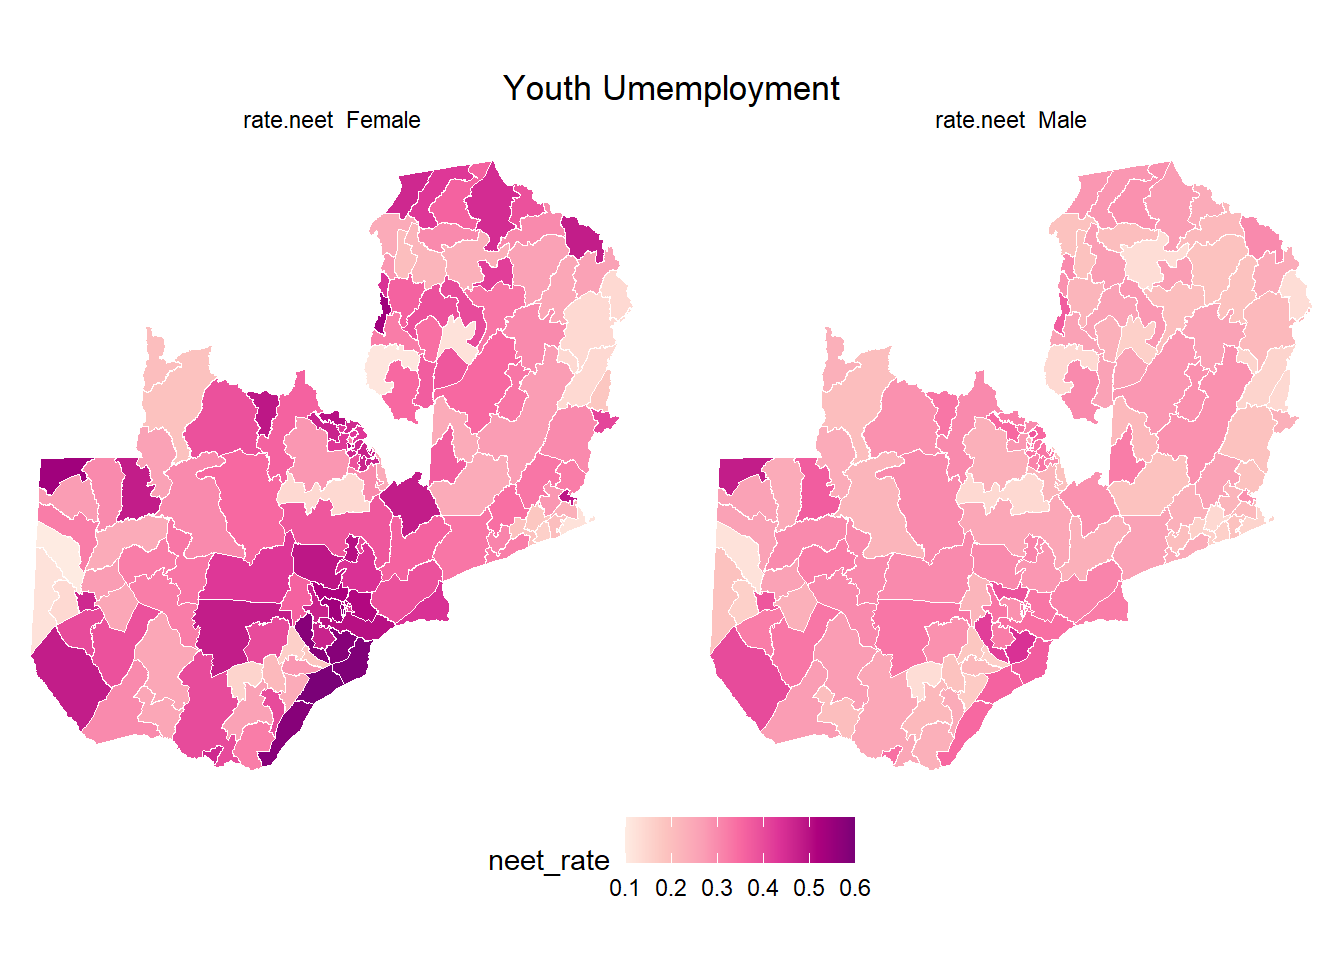
\includegraphics{indicators_notebook_files/figure-latex/unnamed-chunk-13-1.pdf}

\subsection{EXPORT RESULTS SDG RESULTS TO
CSV}\label{export-results-sdg-results-to-csv}

1- Merge all results into one data frame

\begin{Shaded}
\begin{Highlighting}[]
\NormalTok{indicators\_df }\OtherTok{\textless{}{-}} 
\NormalTok{  child\_marriage }\SpecialCharTok{|\textgreater{}}
\NormalTok{  dplyr}\SpecialCharTok{::}\FunctionTok{left\_join}\NormalTok{(}
\NormalTok{    adolescent\_birth\_rate,}
    \AttributeTok{by =} \FunctionTok{c}\NormalTok{(}\StringTok{"CONST\_P\_name"}\NormalTok{, }\StringTok{"CONST\_P"}\NormalTok{)}
\NormalTok{  ) }\SpecialCharTok{|\textgreater{}}
\NormalTok{  dplyr}\SpecialCharTok{::}\FunctionTok{left\_join}\NormalTok{(}
\NormalTok{    youth\_umemplyment,}
    \AttributeTok{by =} \FunctionTok{c}\NormalTok{(}\StringTok{"CONST\_P\_name"}\NormalTok{, }\StringTok{"CONST\_P"}\NormalTok{)}
\NormalTok{  )}
\CommentTok{\# print table}
\NormalTok{indicators\_df }\SpecialCharTok{|\textgreater{}}
  \FunctionTok{head}\NormalTok{() }\SpecialCharTok{|\textgreater{}}
\NormalTok{  gt}\SpecialCharTok{::}\FunctionTok{gt}\NormalTok{()}
\end{Highlighting}
\end{Shaded}

\begin{table}[!t]
\fontsize{12.0pt}{14.4pt}\selectfont
\begin{tabular*}{\linewidth}{@{\extracolsep{\fill}}ccrrrrrrrrrrrrrrrrr}
\toprule
CONST\_P\_name & Constituency & total.girls.20\_24 & married.before.15 & married.before.18 & prop.cm.before.15 & prop.cm.before.18 & total.ado.10\_14 & total.ado.15\_19 & total.ado.birth.10\_14 & total.ado.birth.15\_19 & abr.10\_14 & abr.15\_19 & total.youth.15\_24\_Male & total.youth.15\_24\_Female & total.neet\_Male & total.neet\_Female & rate.neet\_Male & rate.neet\_Female \\ 
\midrule\addlinespace[2.5pt]
Chisamba & 1 & 459 & 9 & 112 & 0.02 & 0.24 & 753 & 622 & 2 & 60 & 2.66 & 96.46 & 1078 & 1081 & 300 & 478 & 0.28 & 0.44 \\ 
Katuba & 2 & 376 & 13 & 101 & 0.03 & 0.27 & 613 & 523 & 0 & 39 & 0.00 & 74.57 & 834 & 899 & 324 & 468 & 0.39 & 0.52 \\ 
Keembe & 3 & 567 & 29 & 176 & 0.05 & 0.31 & 883 & 740 & 4 & 75 & 4.53 & 101.35 & 1227 & 1307 & 365 & 644 & 0.30 & 0.49 \\ 
Bwacha & 4 & 414 & 15 & 91 & 0.04 & 0.22 & 588 & 559 & 0 & 31 & 0.00 & 55.46 & 903 & 973 & 278 & 488 & 0.31 & 0.50 \\ 
Kabwe Central & 5 & 716 & 8 & 85 & 0.01 & 0.12 & 881 & 950 & 6 & 52 & 6.81 & 54.74 & 1444 & 1666 & 437 & 661 & 0.30 & 0.40 \\ 
Kapiri Mposhi & 6 & 1153 & 57 & 344 & 0.05 & 0.30 & 1828 & 1507 & 2 & 140 & 1.09 & 92.90 & 2571 & 2660 & 637 & 1010 & 0.25 & 0.38 \\ 
\bottomrule
\end{tabular*}
\end{table}

2- Export the results into a CSV file for further analysis

\begin{Shaded}
\begin{Highlighting}[]
\NormalTok{readr}\SpecialCharTok{::}\FunctionTok{write\_csv}\NormalTok{(}\AttributeTok{x =}\NormalTok{ indicators\_df, }\AttributeTok{file =} \StringTok{"output/indicators.csv"}\NormalTok{)}
\end{Highlighting}
\end{Shaded}

\subsection{OPTIONAL: APPLICATION OF DEGURBA TO SDG INDICATORS IN
R}\label{optional-application-of-degurba-to-sdg-indicators-in-r}

In this section, we are Going to classify our admin data by DEGURBA
classification generated from the application of the DEGURBA
methodology.

\textbf{Step 0: Classification of Constituencies by DEGURBA}

\begin{Shaded}
\begin{Highlighting}[]
\CommentTok{\# degurba level 1}
\NormalTok{degurba\_l1 }\OtherTok{\textless{}{-}}\NormalTok{ constituency\_shape }\SpecialCharTok{|\textgreater{}}
\NormalTok{  dplyr}\SpecialCharTok{::}\FunctionTok{mutate}\NormalTok{(}
    \AttributeTok{DEGURBA\_L1 =} \FunctionTok{factor}\NormalTok{(DEGURBA\_L1, }
                           \AttributeTok{levels =} \FunctionTok{c}\NormalTok{(}\DecValTok{1}\NormalTok{,}\DecValTok{2}\NormalTok{,}\DecValTok{3}\NormalTok{),}
                           \AttributeTok{labels =} \FunctionTok{c}\NormalTok{(}\StringTok{"Rural Area"}\NormalTok{,}
                                      \StringTok{"Town or Semi{-}dense Area"}\NormalTok{,}
                                      \StringTok{"City"}
\NormalTok{                                      )}
\NormalTok{                           )}
\NormalTok{    ) }\SpecialCharTok{|\textgreater{}}
\NormalTok{  ggplot2}\SpecialCharTok{::}\FunctionTok{ggplot}\NormalTok{() }\SpecialCharTok{+}
\NormalTok{  ggplot2}\SpecialCharTok{::}\FunctionTok{geom\_sf}\NormalTok{(}\FunctionTok{aes}\NormalTok{(}\AttributeTok{fill =}\NormalTok{ DEGURBA\_L1), }\AttributeTok{color =} \StringTok{"white"}\NormalTok{) }\SpecialCharTok{+}
\NormalTok{  ggplot2}\SpecialCharTok{::}\FunctionTok{scale\_fill\_manual}\NormalTok{(}
    \AttributeTok{values =} \FunctionTok{c}\NormalTok{(}\StringTok{"\#375623"}\NormalTok{,}\StringTok{"\#FFC000"}\NormalTok{,}\StringTok{"red"}\NormalTok{)}
\NormalTok{    ) }\SpecialCharTok{+}
\NormalTok{  ggplot2}\SpecialCharTok{::}\FunctionTok{theme\_void}\NormalTok{() }\SpecialCharTok{+}
\NormalTok{  ggplot2}\SpecialCharTok{::}\FunctionTok{labs}\NormalTok{(}\AttributeTok{title =} \StringTok{"DEGURBA LEVEL 1"}\NormalTok{) }\SpecialCharTok{+}
\NormalTok{  ggplot2}\SpecialCharTok{::}\FunctionTok{theme}\NormalTok{(}
    \AttributeTok{plot.title =} \FunctionTok{element\_text}\NormalTok{(}\AttributeTok{face =} \StringTok{"bold"}\NormalTok{)}
\NormalTok{  )}

\CommentTok{\# degurba level 2}
\NormalTok{degurba\_l2 }\OtherTok{\textless{}{-}}\NormalTok{ constituency\_shape }\SpecialCharTok{|\textgreater{}}
\NormalTok{  dplyr}\SpecialCharTok{::}\FunctionTok{mutate}\NormalTok{(}
    \AttributeTok{DEGURBA\_L2 =} \FunctionTok{factor}\NormalTok{(DEGURBA\_L2, }
                           \AttributeTok{levels =} \FunctionTok{c}\NormalTok{(}\DecValTok{11}\NormalTok{,}\DecValTok{12}\NormalTok{,}\DecValTok{13}\NormalTok{,}\DecValTok{21}\NormalTok{,}\DecValTok{23}\NormalTok{,}\DecValTok{30}\NormalTok{), }
                           \AttributeTok{labels =} \FunctionTok{c}\NormalTok{(}\StringTok{"Very Disperded Rural Area"}\NormalTok{,}
                                      \StringTok{"Disperse Rural Area"}\NormalTok{,}
                                      \StringTok{"Village"}\NormalTok{,}
                                      \StringTok{"Suburban or Peri{-}urban Area"}\NormalTok{,}
                                      \StringTok{"Dense Town"}\NormalTok{,}
                                      \StringTok{"City"}
\NormalTok{                                      )}
\NormalTok{                           )}
\NormalTok{    ) }\SpecialCharTok{|\textgreater{}}
\NormalTok{  ggplot2}\SpecialCharTok{::}\FunctionTok{ggplot}\NormalTok{() }\SpecialCharTok{+}
\NormalTok{  ggplot2}\SpecialCharTok{::}\FunctionTok{geom\_sf}\NormalTok{(}\FunctionTok{aes}\NormalTok{(}\AttributeTok{fill =}\NormalTok{ DEGURBA\_L2), }\AttributeTok{color =} \StringTok{"white"}\NormalTok{) }\SpecialCharTok{+}
\NormalTok{  ggplot2}\SpecialCharTok{::}\FunctionTok{scale\_fill\_manual}\NormalTok{(}
    \AttributeTok{values =} \FunctionTok{c}\NormalTok{(}\StringTok{"\#cdf57a"}\NormalTok{,}\StringTok{"\#abcd66"}\NormalTok{,}\StringTok{"\#375623"}\NormalTok{,}\StringTok{"\#ffff00"}\NormalTok{,}\StringTok{"\#732600"}\NormalTok{, }\StringTok{"red"}\NormalTok{)}
\NormalTok{    ) }\SpecialCharTok{+}
\NormalTok{  ggplot2}\SpecialCharTok{::}\FunctionTok{theme\_void}\NormalTok{() }\SpecialCharTok{+}
\NormalTok{  ggplot2}\SpecialCharTok{::}\FunctionTok{labs}\NormalTok{(}\AttributeTok{title =} \StringTok{"DEGURBA LEVEL 2"}\NormalTok{) }\SpecialCharTok{+}
\NormalTok{  ggplot2}\SpecialCharTok{::}\FunctionTok{theme}\NormalTok{(}
    \AttributeTok{plot.title =} \FunctionTok{element\_text}\NormalTok{(}\AttributeTok{face =} \StringTok{"bold"}\NormalTok{)}
\NormalTok{  )}

\CommentTok{\# use patchwork to paste both plot side by side}

\NormalTok{degurba\_l1 }\SpecialCharTok{/}\NormalTok{ degurba\_l2}
\end{Highlighting}
\end{Shaded}

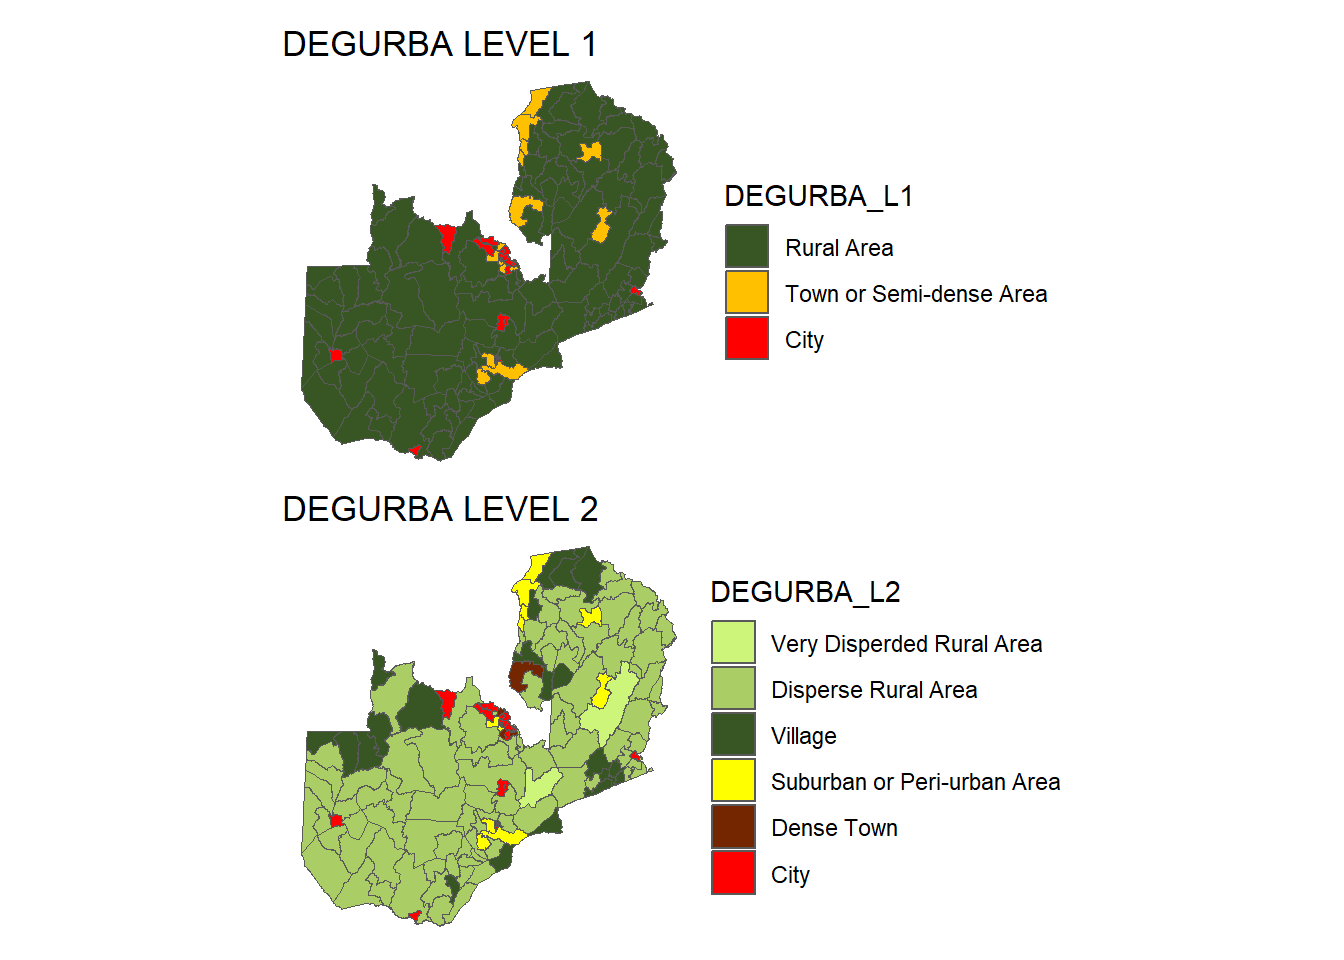
\includegraphics{indicators_notebook_files/figure-latex/unnamed-chunk-16-1.pdf}

\textbf{Step 1: Join the Constituency Shapes and The SDG Indicators}

\begin{Shaded}
\begin{Highlighting}[]
\NormalTok{sdg\_degurba }\OtherTok{\textless{}{-}} 
\NormalTok{  constituency\_shape }\SpecialCharTok{|\textgreater{}}
\NormalTok{  dplyr}\SpecialCharTok{::}\FunctionTok{select}\NormalTok{(NAME1\_, DEGURBA\_L1, DEGURBA\_L2) }\SpecialCharTok{|\textgreater{}}
\NormalTok{  dplyr}\SpecialCharTok{::}\FunctionTok{left\_join}\NormalTok{(}
\NormalTok{    indicators\_df,}
    \AttributeTok{by =} \FunctionTok{c}\NormalTok{(}\StringTok{"NAME1\_"} \OtherTok{=} \StringTok{"CONST\_P\_name"}\NormalTok{)}
\NormalTok{  ) }\SpecialCharTok{|\textgreater{}}
\NormalTok{  tibble}\SpecialCharTok{::}\FunctionTok{as.tibble}\NormalTok{() }\SpecialCharTok{|\textgreater{}}
\NormalTok{  dplyr}\SpecialCharTok{::}\FunctionTok{select}\NormalTok{(}\SpecialCharTok{{-}}\NormalTok{geometry)}

\CommentTok{\# print table}
\NormalTok{sdg\_degurba }\SpecialCharTok{|\textgreater{}}
  \FunctionTok{head}\NormalTok{() }\SpecialCharTok{|\textgreater{}}
\NormalTok{  gt}\SpecialCharTok{::}\FunctionTok{gt}\NormalTok{()}
\end{Highlighting}
\end{Shaded}

\begin{table}[!t]
\fontsize{12.0pt}{14.4pt}\selectfont
\begin{tabular*}{\linewidth}{@{\extracolsep{\fill}}lrrcrrrrrrrrrrrrrrrrr}
\toprule
NAME1\_ & DEGURBA\_L1 & DEGURBA\_L2 & Constituency & total.girls.20\_24 & married.before.15 & married.before.18 & prop.cm.before.15 & prop.cm.before.18 & total.ado.10\_14 & total.ado.15\_19 & total.ado.birth.10\_14 & total.ado.birth.15\_19 & abr.10\_14 & abr.15\_19 & total.youth.15\_24\_Male & total.youth.15\_24\_Female & total.neet\_Male & total.neet\_Female & rate.neet\_Male & rate.neet\_Female \\ 
\midrule\addlinespace[2.5pt]
Itezhi Tezhi & 1 & 12 & 130 & 310 & 13 & 77 & 0.04 & 0.25 & 467 & 427 & 1 & 43 & 2.14 & 100.70 & 671 & 737 & 220 & 357 & 0.33 & 0.48 \\ 
Mulobezi & 1 & 12 & 148 & 135 & 4 & 31 & 0.03 & 0.23 & 223 & 176 & 1 & 16 & 4.48 & 90.91 & 318 & 311 & 86 & 77 & 0.27 & 0.25 \\ 
Sesheke & 1 & 12 & 150 & 213 & 4 & 34 & 0.02 & 0.16 & 277 & 245 & 0 & 13 & 0.00 & 53.06 & 437 & 458 & 119 & 136 & 0.27 & 0.30 \\ 
Sinjembela & 1 & 12 & 147 & 454 & 26 & 143 & 0.06 & 0.31 & 617 & 528 & 0 & 54 & 0.00 & 102.27 & 917 & 982 & 365 & 474 & 0.40 & 0.48 \\ 
Katombola & 1 & 12 & 121 & 463 & 21 & 148 & 0.05 & 0.32 & 758 & 595 & 1 & 54 & 1.32 & 90.76 & 990 & 1058 & 246 & 418 & 0.25 & 0.40 \\ 
Mwandi & 1 & 12 & 149 & 128 & 2 & 23 & 0.02 & 0.18 & 176 & 124 & 0 & 6 & 0.00 & 48.39 & 226 & 252 & 46 & 64 & 0.20 & 0.25 \\ 
\bottomrule
\end{tabular*}
\end{table}

\textbf{Step 2 : SDG dissagregation by DEGURBA}

\begin{Shaded}
\begin{Highlighting}[]
\NormalTok{sdg\_degurba\_diss }\OtherTok{\textless{}{-}} 
\NormalTok{  sdg\_degurba }\SpecialCharTok{|\textgreater{}}
\NormalTok{  tidyr}\SpecialCharTok{::}\FunctionTok{pivot\_longer}\NormalTok{(}
    \AttributeTok{cols =} \FunctionTok{c}\NormalTok{(}\StringTok{"DEGURBA\_L1"}\NormalTok{, }\StringTok{"DEGURBA\_L2"}\NormalTok{),}
    \AttributeTok{names\_to =} \StringTok{"degurba\_level"}\NormalTok{,}
    \AttributeTok{values\_to =} \StringTok{"degurba\_class"}
\NormalTok{  ) }\SpecialCharTok{|\textgreater{}}
\NormalTok{  dplyr}\SpecialCharTok{::}\FunctionTok{group\_by}\NormalTok{(degurba\_level, degurba\_class) }\SpecialCharTok{|\textgreater{}}
\NormalTok{  dplyr}\SpecialCharTok{::}\FunctionTok{summarise}\NormalTok{(}
    \AttributeTok{total.girls.20\_24 =} \FunctionTok{sum}\NormalTok{(total.girls}\FloatTok{.20}\NormalTok{\_24),}
    \AttributeTok{married.before.15   =} \FunctionTok{sum}\NormalTok{(married.before}\FloatTok{.15}\NormalTok{),}
    \AttributeTok{married.before.18 =} \FunctionTok{sum}\NormalTok{(married.before}\FloatTok{.18}\NormalTok{),}
    \AttributeTok{prop.cm.before.15   =} \FunctionTok{round}\NormalTok{((married.before}\FloatTok{.15} \SpecialCharTok{/}\NormalTok{ total.girls}\FloatTok{.20}\NormalTok{\_24), }\DecValTok{2}\NormalTok{),}
    \AttributeTok{prop.cm.before.18 =} \FunctionTok{round}\NormalTok{((married.before}\FloatTok{.18} \SpecialCharTok{/}\NormalTok{ total.girls}\FloatTok{.20}\NormalTok{\_24), }\DecValTok{2}\NormalTok{),}
    \AttributeTok{total.ado.10\_14 =} \FunctionTok{sum}\NormalTok{(total.ado}\FloatTok{.10}\NormalTok{\_14),}
    \AttributeTok{total.ado.15\_19 =} \FunctionTok{sum}\NormalTok{(total.ado}\FloatTok{.15}\NormalTok{\_19),}
    \AttributeTok{total.ado.birth.10\_14   =} \FunctionTok{sum}\NormalTok{(total.ado.birth}\FloatTok{.10}\NormalTok{\_14),}
    \AttributeTok{total.ado.birth.15\_19   =} \FunctionTok{sum}\NormalTok{(total.ado.birth}\FloatTok{.15}\NormalTok{\_19),}
    \AttributeTok{abr.10\_14   =} \FunctionTok{round}\NormalTok{((total.ado.birth}\FloatTok{.10}\NormalTok{\_14}\SpecialCharTok{/}\NormalTok{total.ado}\FloatTok{.10}\NormalTok{\_14)}\SpecialCharTok{*}\DecValTok{1000}\NormalTok{, }\DecValTok{2}\NormalTok{),}
    \AttributeTok{abr.15\_19   =} \FunctionTok{round}\NormalTok{((total.ado.birth}\FloatTok{.15}\NormalTok{\_19}\SpecialCharTok{/}\NormalTok{total.ado}\FloatTok{.15}\NormalTok{\_19)}\SpecialCharTok{*}\DecValTok{1000}\NormalTok{, }\DecValTok{2}\NormalTok{),}
    \AttributeTok{total.youth.15\_24\_Male =} \FunctionTok{sum}\NormalTok{(total.youth}\FloatTok{.15}\NormalTok{\_24\_Male),}
    \AttributeTok{total.youth.15\_24\_Female =} \FunctionTok{sum}\NormalTok{(total.youth}\FloatTok{.15}\NormalTok{\_24\_Female),}
    \AttributeTok{total.neet\_Male =} \FunctionTok{sum}\NormalTok{(total.neet\_Male),}
    \AttributeTok{total.neet\_Female   =} \FunctionTok{sum}\NormalTok{(total.neet\_Female),}
    \AttributeTok{rate.neet\_Male =} \FunctionTok{round}\NormalTok{((total.neet\_Male }\SpecialCharTok{/}\NormalTok{ total.youth}\FloatTok{.15}\NormalTok{\_24\_Male), }\DecValTok{2}\NormalTok{),}
    \AttributeTok{rate.neet\_Female =} \FunctionTok{round}\NormalTok{((total.youth}\FloatTok{.15}\NormalTok{\_24\_Female }\SpecialCharTok{/}\NormalTok{ total.neet\_Female), }\DecValTok{2}\NormalTok{)}
\NormalTok{  )}


\NormalTok{sdg\_degurba\_diss }\OtherTok{\textless{}{-}} 
\NormalTok{  sdg\_degurba\_diss }\SpecialCharTok{|\textgreater{}}
\NormalTok{  dplyr}\SpecialCharTok{::}\FunctionTok{mutate}\NormalTok{(}
    \AttributeTok{degurba\_class =} \FunctionTok{factor}\NormalTok{(degurba\_class, }
                           \AttributeTok{levels =} \FunctionTok{c}\NormalTok{(}\DecValTok{1}\NormalTok{,}\DecValTok{2}\NormalTok{,}\DecValTok{3}\NormalTok{,}\DecValTok{11}\NormalTok{,}\DecValTok{12}\NormalTok{,}\DecValTok{13}\NormalTok{,}\DecValTok{21}\NormalTok{,}\DecValTok{23}\NormalTok{,}\DecValTok{30}\NormalTok{), }
                           \AttributeTok{labels =} \FunctionTok{c}\NormalTok{(}\StringTok{"Rural Area"}\NormalTok{,}
                                      \StringTok{"Town or Semi{-}dense Area"}\NormalTok{,}
                                      \StringTok{"City"}\NormalTok{,}
                                      \StringTok{"Very Disperded Rural Area"}\NormalTok{,}
                                      \StringTok{"Disperse Rural Area"}\NormalTok{,}
                                      \StringTok{"Village"}\NormalTok{,}
                                      \StringTok{"Suburban or Peri{-}urban Area"}\NormalTok{,}
                                      \StringTok{"Dense Town"}\NormalTok{,}
                                      \StringTok{"city"}
\NormalTok{                                      )}
\NormalTok{                           )}
\NormalTok{    )}
\end{Highlighting}
\end{Shaded}

\textbf{Step 3: Visualization}

\begin{Shaded}
\begin{Highlighting}[]
\NormalTok{sdg\_degurba\_diss }\SpecialCharTok{|\textgreater{}}
\NormalTok{  gt}\SpecialCharTok{::}\FunctionTok{gt}\NormalTok{() }\SpecialCharTok{|\textgreater{}}
\NormalTok{  gt}\SpecialCharTok{::}\FunctionTok{tab\_header}\NormalTok{(}\AttributeTok{title =} \StringTok{"SDG INDICATOR BY DEGURBA"}\NormalTok{,}
                 \AttributeTok{subtitle =} \StringTok{"Zambia 2010 Pop \& House Census"}\NormalTok{) }\SpecialCharTok{|\textgreater{}}
\NormalTok{  gt}\SpecialCharTok{::}\FunctionTok{data\_color}\NormalTok{(}
    \AttributeTok{columns =} \FunctionTok{c}\NormalTok{(}\StringTok{"prop.cm.before.15"}\NormalTok{,    }
                \StringTok{"prop.cm.before.18"}
\NormalTok{                ),}
    \AttributeTok{method =} \StringTok{"numeric"}\NormalTok{,}
    \AttributeTok{palette =} \StringTok{"OrRd"}\NormalTok{,}
    \AttributeTok{domain =} \FunctionTok{c}\NormalTok{(}\FunctionTok{min}\NormalTok{(sdg\_degurba\_diss}\SpecialCharTok{$}\NormalTok{prop.cm.before}\FloatTok{.15}\NormalTok{), }
               \FunctionTok{max}\NormalTok{(sdg\_degurba\_diss}\SpecialCharTok{$}\NormalTok{prop.cm.before}\FloatTok{.18}\NormalTok{))}
\NormalTok{  ) }\SpecialCharTok{|\textgreater{}}
\NormalTok{  gt}\SpecialCharTok{::}\FunctionTok{data\_color}\NormalTok{(}
    \AttributeTok{columns =} \FunctionTok{c}\NormalTok{(}\StringTok{"abr.10\_14"}\NormalTok{, }
                \StringTok{"abr.15\_19"}
\NormalTok{                ),}
    \AttributeTok{method =} \StringTok{"numeric"}\NormalTok{,}
    \AttributeTok{palette =} \StringTok{"OrRd"}\NormalTok{,}
    \AttributeTok{domain =} \FunctionTok{c}\NormalTok{(}\FunctionTok{min}\NormalTok{(sdg\_degurba\_diss}\SpecialCharTok{$}\NormalTok{abr}\FloatTok{.10}\NormalTok{\_14), }
               \FunctionTok{max}\NormalTok{(sdg\_degurba\_diss}\SpecialCharTok{$}\NormalTok{abr}\FloatTok{.15}\NormalTok{\_19))}
\NormalTok{  ) }\SpecialCharTok{|\textgreater{}}
\NormalTok{  gt}\SpecialCharTok{::}\FunctionTok{data\_color}\NormalTok{(}
    \AttributeTok{columns =} \FunctionTok{c}\NormalTok{(}\StringTok{"rate.neet\_Male"}\NormalTok{, }
                \StringTok{"rate.neet\_Female"}
\NormalTok{                ),}
    \AttributeTok{method =} \StringTok{"numeric"}\NormalTok{,}
    \AttributeTok{palette =} \StringTok{"OrRd"}\NormalTok{,}
    \AttributeTok{domain =} \FunctionTok{c}\NormalTok{(}\FunctionTok{min}\NormalTok{(sdg\_degurba\_diss}\SpecialCharTok{$}\NormalTok{rate.neet\_Male), }
               \FunctionTok{max}\NormalTok{(sdg\_degurba\_diss}\SpecialCharTok{$}\NormalTok{rate.neet\_Female))}
\NormalTok{  ) }\SpecialCharTok{|\textgreater{}}
  \FunctionTok{tab\_style}\NormalTok{(}
    \AttributeTok{style =} \FunctionTok{list}\NormalTok{(}
      \FunctionTok{cell\_fill}\NormalTok{(}\AttributeTok{color =} \StringTok{"\#375623"}\NormalTok{) }
\NormalTok{      ),}
    \AttributeTok{locations =} \FunctionTok{cells\_body}\NormalTok{(}
      \AttributeTok{columns =}\NormalTok{ degurba\_class,}
      \AttributeTok{rows =}\NormalTok{ degurba\_class }\SpecialCharTok{\%in\%} \FunctionTok{c}\NormalTok{(}\StringTok{"Rural Area"}\NormalTok{, }\StringTok{"Village"}\NormalTok{)}
\NormalTok{      )}
\NormalTok{  ) }\SpecialCharTok{|\textgreater{}}
  \FunctionTok{tab\_style}\NormalTok{(}
    \AttributeTok{style =} \FunctionTok{list}\NormalTok{(}
      \FunctionTok{cell\_fill}\NormalTok{(}\AttributeTok{color =} \StringTok{"\#FFC000"}\NormalTok{) }
\NormalTok{      ),}
    \AttributeTok{locations =} \FunctionTok{cells\_body}\NormalTok{(}
      \AttributeTok{columns =}\NormalTok{ degurba\_class,}
      \AttributeTok{rows =}\NormalTok{ degurba\_class }\SpecialCharTok{==} \StringTok{"Town or Semi{-}dense Area"}
\NormalTok{    )}
\NormalTok{  ) }\SpecialCharTok{|\textgreater{}}
  \FunctionTok{tab\_style}\NormalTok{(}
    \AttributeTok{style =} \FunctionTok{list}\NormalTok{(}
      \FunctionTok{cell\_fill}\NormalTok{(}\AttributeTok{color =} \StringTok{"red"}\NormalTok{)}
\NormalTok{      ),}
    \AttributeTok{locations =} \FunctionTok{cells\_body}\NormalTok{(}
      \AttributeTok{columns =}\NormalTok{ degurba\_class,}
      \AttributeTok{rows =}\NormalTok{ degurba\_class }\SpecialCharTok{\%in\%} \FunctionTok{c}\NormalTok{(}\StringTok{"City"}\NormalTok{, }\StringTok{"city"}\NormalTok{)}
\NormalTok{    )}
\NormalTok{  ) }\SpecialCharTok{|\textgreater{}}
  \FunctionTok{tab\_style}\NormalTok{(}
    \AttributeTok{style =} \FunctionTok{list}\NormalTok{(}
      \FunctionTok{cell\_fill}\NormalTok{(}\AttributeTok{color =} \StringTok{"\#cdf57a"}\NormalTok{)}
\NormalTok{      ),}
    \AttributeTok{locations =} \FunctionTok{cells\_body}\NormalTok{(}
      \AttributeTok{columns =}\NormalTok{ degurba\_class,}
      \AttributeTok{rows =}\NormalTok{ degurba\_class }\SpecialCharTok{==} \StringTok{"Very Disperded Rural Area"}
\NormalTok{    )}
\NormalTok{  ) }\SpecialCharTok{|\textgreater{}}
  \FunctionTok{tab\_style}\NormalTok{(}
    \AttributeTok{style =} \FunctionTok{list}\NormalTok{(}
      \FunctionTok{cell\_fill}\NormalTok{(}\AttributeTok{color =} \StringTok{"\#abcd66"}\NormalTok{)}
\NormalTok{      ),}
    \AttributeTok{locations =} \FunctionTok{cells\_body}\NormalTok{(}
      \AttributeTok{columns =}\NormalTok{ degurba\_class,}
      \AttributeTok{rows =}\NormalTok{ degurba\_class }\SpecialCharTok{==} \StringTok{"Disperse Rural Area"}
\NormalTok{    )}
\NormalTok{  ) }\SpecialCharTok{|\textgreater{}}
  \FunctionTok{tab\_style}\NormalTok{(}
    \AttributeTok{style =} \FunctionTok{list}\NormalTok{(}
      \FunctionTok{cell\_fill}\NormalTok{(}\AttributeTok{color =} \StringTok{"\#ffff00"}\NormalTok{)}
\NormalTok{      ),}
    \AttributeTok{locations =} \FunctionTok{cells\_body}\NormalTok{(}
      \AttributeTok{columns =}\NormalTok{ degurba\_class,}
      \AttributeTok{rows =}\NormalTok{ degurba\_class }\SpecialCharTok{==} \StringTok{"Suburban or Peri{-}urban Area"}
\NormalTok{    )}
\NormalTok{  ) }\SpecialCharTok{|\textgreater{}}
  \FunctionTok{tab\_style}\NormalTok{(}
    \AttributeTok{style =} \FunctionTok{list}\NormalTok{(}
      \FunctionTok{cell\_fill}\NormalTok{(}\AttributeTok{color =} \StringTok{"\#732600"}\NormalTok{)}
\NormalTok{      ),}
    \AttributeTok{locations =} \FunctionTok{cells\_body}\NormalTok{(}
      \AttributeTok{columns =}\NormalTok{ degurba\_class,}
      \AttributeTok{rows =}\NormalTok{ degurba\_class }\SpecialCharTok{==} \StringTok{"Dense Town"}
\NormalTok{    )}
\NormalTok{  )}
\end{Highlighting}
\end{Shaded}

\begin{table}[!t]
\caption*{
{\large SDG INDICATOR BY DEGURBA} \\ 
{\small Zambia 2010 Pop \& House Census}
} 
\fontsize{12.0pt}{14.4pt}\selectfont
\begin{tabular*}{\linewidth}{@{\extracolsep{\fill}}crrrrrrrrrrrrrrrrr}
\toprule
degurba\_class & total.girls.20\_24 & married.before.15 & married.before.18 & prop.cm.before.15 & prop.cm.before.18 & total.ado.10\_14 & total.ado.15\_19 & total.ado.birth.10\_14 & total.ado.birth.15\_19 & abr.10\_14 & abr.15\_19 & total.youth.15\_24\_Male & total.youth.15\_24\_Female & total.neet\_Male & total.neet\_Female & rate.neet\_Male & rate.neet\_Female \\ 
\midrule\addlinespace[2.5pt]
\multicolumn{18}{l}{DEGURBA\_L1} \\[2.5pt] 
\midrule\addlinespace[2.5pt]
{\cellcolor[HTML]{375623}{Rural Area}} & 37060 & 1822 & 11142 & {\cellcolor[HTML]{FFEDD4}{\textcolor[HTML]{000000}{0.05}}} & {\cellcolor[HTML]{CF2818}{\textcolor[HTML]{FFFFFF}{0.30}}} & 56187 & 46653 & 116 & 4296 & {\cellcolor[HTML]{FFF4E6}{\textcolor[HTML]{000000}{2.06}}} & {\cellcolor[HTML]{850000}{\textcolor[HTML]{FFFFFF}{92.08}}} & 78193 & 83713 & 19677 & 28367 & {\cellcolor[HTML]{FFF7EC}{\textcolor[HTML]{000000}{0.25}}} & {\cellcolor[HTML]{A20001}{\textcolor[HTML]{FFFFFF}{2.95}}} \\ 
{\cellcolor[HTML]{FFC000}{Town or Semi-dense Area}} & 6963 & 284 & 1628 & {\cellcolor[HTML]{FFF0DC}{\textcolor[HTML]{000000}{0.04}}} & {\cellcolor[HTML]{F4734E}{\textcolor[HTML]{FFFFFF}{0.23}}} & 9724 & 8772 & 27 & 678 & {\cellcolor[HTML]{FFF3E3}{\textcolor[HTML]{000000}{2.78}}} & {\cellcolor[HTML]{C1180C}{\textcolor[HTML]{FFFFFF}{77.29}}} & 14386 & 15735 & 4113 & 6581 & {\cellcolor[HTML]{FFF5E8}{\textcolor[HTML]{000000}{0.29}}} & {\cellcolor[HTML]{DC3C27}{\textcolor[HTML]{FFFFFF}{2.39}}} \\ 
{\cellcolor[HTML]{FF0000}{City}} & 21146 & 423 & 3272 & {\cellcolor[HTML]{FFF7EC}{\textcolor[HTML]{000000}{0.02}}} & {\cellcolor[HTML]{FDBE87}{\textcolor[HTML]{000000}{0.15}}} & 24177 & 23791 & 61 & 1272 & {\cellcolor[HTML]{FFF4E4}{\textcolor[HTML]{000000}{2.52}}} & {\cellcolor[HTML]{F5774F}{\textcolor[HTML]{FFFFFF}{53.47}}} & 38909 & 44937 & 12878 & 21757 & {\cellcolor[HTML]{FFF4E4}{\textcolor[HTML]{000000}{0.33}}} & {\cellcolor[HTML]{F06849}{\textcolor[HTML]{FFFFFF}{2.07}}} \\ 
\midrule\addlinespace[2.5pt]
\multicolumn{18}{l}{DEGURBA\_L2} \\[2.5pt] 
\midrule\addlinespace[2.5pt]
{\cellcolor[HTML]{CDF57A}{Very Disperded Rural Area}} & 265 & 27 & 102 & {\cellcolor[HTML]{FDD8A7}{\textcolor[HTML]{000000}{0.10}}} & {\cellcolor[HTML]{7F0000}{\textcolor[HTML]{FFFFFF}{0.38}}} & 349 & 286 & 0 & 20 & {\cellcolor[HTML]{FFF7EC}{\textcolor[HTML]{000000}{0.00}}} & {\cellcolor[HTML]{D73120}{\textcolor[HTML]{FFFFFF}{69.93}}} & 459 & 551 & 119 & 172 & {\cellcolor[HTML]{FFF7EB}{\textcolor[HTML]{000000}{0.26}}} & {\cellcolor[HTML]{7F0000}{\textcolor[HTML]{FFFFFF}{3.20}}} \\ 
{\cellcolor[HTML]{ABCD66}{Disperse Rural Area}} & 29834 & 1412 & 8907 & {\cellcolor[HTML]{FFEDD4}{\textcolor[HTML]{000000}{0.05}}} & {\cellcolor[HTML]{CF2818}{\textcolor[HTML]{FFFFFF}{0.30}}} & 45485 & 37743 & 84 & 3529 & {\cellcolor[HTML]{FFF5E6}{\textcolor[HTML]{000000}{1.85}}} & {\cellcolor[HTML]{7F0000}{\textcolor[HTML]{FFFFFF}{93.50}}} & 63143 & 67577 & 15876 & 22793 & {\cellcolor[HTML]{FFF7EC}{\textcolor[HTML]{000000}{0.25}}} & {\cellcolor[HTML]{A00001}{\textcolor[HTML]{FFFFFF}{2.96}}} \\ 
{\cellcolor[HTML]{375623}{Village}} & 6961 & 383 & 2133 & {\cellcolor[HTML]{FEEACC}{\textcolor[HTML]{000000}{0.06}}} & {\cellcolor[HTML]{C72012}{\textcolor[HTML]{FFFFFF}{0.31}}} & 10353 & 8624 & 32 & 747 & {\cellcolor[HTML]{FFF3E2}{\textcolor[HTML]{000000}{3.09}}} & {\cellcolor[HTML]{9D0001}{\textcolor[HTML]{FFFFFF}{86.62}}} & 14591 & 15585 & 3682 & 5402 & {\cellcolor[HTML]{FFF7EC}{\textcolor[HTML]{000000}{0.25}}} & {\cellcolor[HTML]{AA0001}{\textcolor[HTML]{FFFFFF}{2.89}}} \\ 
{\cellcolor[HTML]{FFFF00}{Suburban or Peri-urban Area}} & 5663 & 254 & 1428 & {\cellcolor[HTML]{FFF0DC}{\textcolor[HTML]{000000}{0.04}}} & {\cellcolor[HTML]{EC6043}{\textcolor[HTML]{FFFFFF}{0.25}}} & 7920 & 6862 & 20 & 574 & {\cellcolor[HTML]{FFF4E4}{\textcolor[HTML]{000000}{2.53}}} & {\cellcolor[HTML]{AB0001}{\textcolor[HTML]{FFFFFF}{83.65}}} & 11441 & 12525 & 3273 & 5299 & {\cellcolor[HTML]{FFF5E8}{\textcolor[HTML]{000000}{0.29}}} & {\cellcolor[HTML]{DE412A}{\textcolor[HTML]{FFFFFF}{2.36}}} \\ 
{\cellcolor[HTML]{732600}{Dense Town}} & 1300 & 30 & 200 & {\cellcolor[HTML]{FFF7EC}{\textcolor[HTML]{000000}{0.02}}} & {\cellcolor[HTML]{FDBE87}{\textcolor[HTML]{000000}{0.15}}} & 1804 & 1910 & 7 & 104 & {\cellcolor[HTML]{FFF2E0}{\textcolor[HTML]{000000}{3.88}}} & {\cellcolor[HTML]{F4734E}{\textcolor[HTML]{FFFFFF}{54.45}}} & 2945 & 3210 & 840 & 1282 & {\cellcolor[HTML]{FFF5E8}{\textcolor[HTML]{000000}{0.29}}} & {\cellcolor[HTML]{D32C1C}{\textcolor[HTML]{FFFFFF}{2.50}}} \\ 
{\cellcolor[HTML]{FF0000}{city}} & 21146 & 423 & 3272 & {\cellcolor[HTML]{FFF7EC}{\textcolor[HTML]{000000}{0.02}}} & {\cellcolor[HTML]{FDBE87}{\textcolor[HTML]{000000}{0.15}}} & 24177 & 23791 & 61 & 1272 & {\cellcolor[HTML]{FFF4E4}{\textcolor[HTML]{000000}{2.52}}} & {\cellcolor[HTML]{F5774F}{\textcolor[HTML]{FFFFFF}{53.47}}} & 38909 & 44937 & 12878 & 21757 & {\cellcolor[HTML]{FFF4E4}{\textcolor[HTML]{000000}{0.33}}} & {\cellcolor[HTML]{F06849}{\textcolor[HTML]{FFFFFF}{2.07}}} \\ 
\bottomrule
\end{tabular*}
\end{table}

\end{document}
